\documentclass[12pt,onecolumn,a4paper]{IEEEtran}
\usepackage[T1]{fontenc}

% ==========================================================================
% PREAMBLE AND PACKAGES
% ==========================================================================
\usepackage{amsmath,amssymb,amsfonts} 
\usepackage{booktabs}           
\usepackage{geometry}           
\usepackage{hyperref}           
\usepackage{setspace}           
\usepackage{graphicx}           
\usepackage{array}              
\usepackage{caption}            
\usepackage{subcaption}         
\usepackage{listings}           
\usepackage{color}              
\usepackage{enumitem}           
\usepackage{fancyhdr}           
\usepackage{cite}               
\usepackage{bm}                 
\usepackage{indentfirst}        
\usepackage{algorithm}          
\usepackage{algpseudocode}      


% ==========================================================================
% PAGE CONFIGURATION
% ==========================================================================
\geometry{margin=1in}
\setstretch{1.4}

\hypersetup{
    colorlinks=true,
    linkcolor=red,
    citecolor=green,
    filecolor=magenta,      
    urlcolor=blue,
    pdftitle={Thesis - Brhanu Atsbaha - Multi-modal Historical Image Analysis},
    pdfpagemode=FullScreen,
}

% ==========================================================================
% HEADER AND FOOTER DEFINITIONS
% ==========================================================================
\setlength{\headheight}{14pt}
\pagestyle{fancy}
\fancyhf{}
\rhead{Brhanu Atsbaha}
\lhead{Computer Vision for Historic Archives}
\cfoot{\thepage}

% ==========================================================================
% TITLE DATA
% ==========================================================================
\title{\Huge \textbf{Multi-Agent Visual Analysis for Historic Archives: Object and Complex Scene Detection with Cross-Modal Validation} \\ [0.5cm]
\Large \textbf{A Complementary Agent Framework Combining Restoration, Grounding, Reasoning, and Human-in-the-Loop Verification}}

\author{\large Brhanu Atsbaha \\ 
\textit{Masters in Data Analytics} \\ 
University of Hildesheim, Germany \\
Supervised by: Prof. Dr. Thomas Mandl \\
}

\date{Feb 20, 2026}

\begin{document}
\maketitle

% ==========================================================================
% ABSTRACT
% ==========================================================================
\begin{abstract}
This thesis addresses automated object and complex scene detection in historical archives under severe domain shift, sparse labels, and heterogeneous degradation. Rather than treating the task as a single-model prediction problem, we formulate it as a \textbf{multi-agent validation system} in which complementary modalities provide independent evidence of scene realism and semantic consistency.

We introduce \textit{Visual Historian-MAS}, a coordinated architecture composed of specialized agents: (i) restoration agents (CycleGAN \cite{cyclegan2017}, Real-ESRGAN \cite{realesrgan2021}, diffusion refinement \cite{stable_diffusion2022}), (ii) object-grounding agents (GroundingDINO \cite{groundingdino2023}, Florence-2 \cite{florence2_2023}, YOLOv11 student \cite{yolov11_2024}), (iii) scene and reasoning agents (CLIP/SigLIP scene priors \cite{clip2021,siglip2023}, LLaVA-OneVision), and (iv) a document/layout agent (Kosmos-2.5 \cite{kosmos2_5_2024}). A coordinator fuses agent outputs via agreement- and uncertainty-aware scoring and routes ambiguous samples to human review.

The central contribution is a validation-centric protocol for complex archival scenes: realism is inferred from cross-agent agreement patterns, disagreement is used as an uncertainty signal, and human-in-the-loop triage is prioritized by agent conflict. This enables robust indexing beyond detector confidence alone and supports reproducible archival analytics across 12,110 images.

The thesis reports architectural evolution, agent ablations, and agreement-based analyses, and provides a production-oriented implementation for scalable digital heritage workflows where AI outputs are treated as evidence to be validated, not as unquestioned ground truth.
\end{abstract}

\newpage
\tableofcontents
\newpage
\listoffigures
\newpage
\listoftables
\newpage

% ==========================================================================
% SECTION 1: INTRODUCTION
% ==========================================================================
\section{Introduction}
\subsection{The Archival Challenge in the Digital Age}
Historical illustrations are critical primary sources for historians, sociologists, 
and cultural researchers. They capture moments of social change, architectural 
evolution, and daily life that are nowhere else documented in such visual detail. 

However, the sheer volume of digitized archives makes manual cataloging impossible. 
 In the Colibri Historical Image Collection, which contains over 53,000 images, the lack of dual-modality (visual and textual) searchability significantly hampers the discovery of specific historical events and figures.
\subsection{Identification of the Research Gap}
While modern object detection has reached human-level performance on benchmarks 
like COCO \cite{coco2014} or OpenImages \cite{openimages2020}, these models rely on "High-Fidelity" samples. 
Historical illustrations exist in a "Low-Fidelity" regime characterized by several distinct degradation factors. 
However, it is important to note that while camera blur is often cited as a degradation factor in modern computer vision, historical archives frequently contain fewer "action" illustrations compared to modern datasets. In early illustrations, blur is more often a result of slow lens speeds and physical camera instability rather than subject motion.

The primary research gap addressed in this work is the lack of a unified, restorative pipeline that can bridge the gap between these legacy scans and the high-fidelity features required for state-of-the-art detection.

\subsection{Research Objectives and Goals}
The overarching goal of this research is to bridge the "archival semantic gap" through a reproducible \textbf{multi-agent} framework for historical indexing and validation. By establishing the \textit{Visual Historian-MAS} platform, we transform raw legacy scans into evidence-rich semantic records. Specifically, this work addresses the following research questions:
\begin{itemize}
    \item \textbf{RQ1 -- Multi-Agent Reliability}: Does multi-agent cross-modal validation improve object and scene reliability over single-model baselines in historical archives?
    \item \textbf{RQ2 -- Uncertainty from Disagreement}: Are inter-agent disagreement patterns better predictors of annotation error and realism failure than model confidence alone?
    \item \textbf{RQ3 -- Agent Complementarity}: Which combinations of object, scene, reasoning, and document agents contribute most on complex scenes (occlusion, clutter, low contrast)?
    \item \textbf{RQ4 -- Human-in-the-Loop Efficiency}: Can disagreement-driven triage reduce manual validation effort while preserving or improving metadata quality?
\end{itemize}

\subsection{Evaluation Methodology for Multi-Agent Analysis}
The evaluation protocol is designed to isolate both predictive quality and validation quality:
\begin{itemize}
    \item \textbf{Single-Agent Baselines}: Evaluate each agent independently (object detector, scene classifier, VLM reasoning, document/OCR) using standard metrics for its task.
    \item \textbf{Coordinator Evaluation}: Compare weighted multi-agent fusion against single-agent baselines using agreement, realism score distributions, and downstream indexing quality.
    \item \textbf{Ablation Analysis}: Remove one agent at a time and measure degradation in agreement, realism confidence, and review precision.
    \item \textbf{Complex-Scene Stratification}: Report performance separately for high clutter, low contrast, and high-occlusion subsets.
    \item \textbf{HITL Efficiency}: Quantify precision@k of disagreement-based triage and estimate reviewer effort reduction against random sampling.
\end{itemize}

\subsubsection{Measured vs. Proxy Provenance Policy}
To ensure methodological transparency, all reported metrics are tagged by provenance:
\begin{itemize}
    \item \textbf{Measured}: Derived directly from persisted model artifacts (e.g., explicit score files, annotated benchmarks).
    \item \textbf{Proxy}: Computed fallback estimates used only when measured artifacts are unavailable.
    \item \textbf{Mixed}: Composite metrics where at least one component is proxy-derived.
\end{itemize}
All result tables in this thesis follow this policy and explicitly report source tags (e.g., \texttt{agreement\_source}, \texttt{metric\_source}) to avoid over-claiming from fallback signals.

\subsection{State of the Art in Historical Image Analysis}
Recent years have seen a significant methodological shift in computational cultural heritage research. Rather than treating historical imagery as a mere variant of natural images, modern studies increasingly recognize archives as a distinct visual domain characterized by degradation, stylistic divergence, and annotation scarcity. This section situates the Visual Historian-MAS framework within this emerging research landscape.

\subsubsection{Object Detection Under Historical Domain Shift}
Traditional object detectors trained on modern benchmarks such as COCO \cite{coco2014} assume high-resolution, color-consistent imagery with stable texture statistics. Historical illustrations violate these assumptions due to film grain, chemical artifacts, fading, and monochromatic capture. Consequently, detectors exhibit severe performance degradation when directly applied to archives.

Kim et al.~\cite{kim2024historical_od} present one of the most directly aligned studies with this thesis. Their work addresses object detection in historical illustrations through a two-stage adaptation strategy. First, modern labeled datasets are translated into the visual style of historical imagery using CycleGAN, effectively synthesizing domain-aligned training samples. Second, pseudo-labeling is employed to iteratively expand supervision without manual annotation. Their findings demonstrate that generative domain translation can substantially reduce the annotation burden while preserving detector performance.

This thesis extends that paradigm beyond dataset adaptation by introducing a restoration-first architecture. Rather than adapting modern images into historical style, we normalize degraded archival scans into a statistically modern visual regime, improving compatibility with foundational Vision-Language Models (VLMs). Conceptually, Kim et al.~optimize the training distribution, whereas Visual Historian-MAS optimizes the inference distribution and cross-agent validation.

\subsubsection{Surveyed Challenges in Visual-Art Object Detection}
While historical illustrations represent one form of domain shift, visual art datasets introduce even greater depictive variability. Bengamra et al.~\cite{bengamra2024survey_visualart_od} provide a comprehensive survey of object detection methods in visual art, proposing a taxonomy organized by supervision level, detection frameworks, and representation challenges. Their study identifies three persistent technical obstacles:

\begin{itemize}
    \item \textbf{Depictive Domain Gap}: Differences between artistic and photographic representations.
    \item \textbf{Annotation Ambiguity}: Lack of consistent object definitions across datasets.
    \item \textbf{Metric Instability}: Difficulty evaluating detectors on stylistically diverse corpora.
\end{itemize}

Although focused primarily on paintings and artworks, these challenges map directly onto historical archives. Degradation artifacts function analogously to stylistic abstraction, distorting edge and texture features. Furthermore, annotation ambiguity is intrinsic to archives where object categories are historically contingent. The survey reinforces the necessity of robust domain normalization and open-vocabulary detection strategies --- central design principles of the multi-agent framework.

\subsubsection{Foundation Models and Epistemic Reframing in Digital Art History}
Recent discourse in digital humanities increasingly interrogates the epistemological implications of large-scale foundation models. Impett and Offert~\cite{impett_offert_2022_dah} argue that transformer-based vision architectures implicitly encode a cultural model of visuality derived from web-scale datasets. These models do not merely detect objects; they operationalize historically situated visual categories learned from contemporary imagery.

This perspective is critical when applying VLMs to historical archives. Predictions may reflect modern semantic priors rather than historically accurate interpretations. The authors therefore advocate for critical, interpretable AI workflows where outputs are treated as analytical propositions rather than objective truths.

Visual Historian-MAS adopts this philosophy through its consensus principle. Multi-agent agreement, confidence thresholds, and interactive verification interfaces explicitly acknowledge epistemic uncertainty. Rather than assuming model correctness, the system quantifies model belief consistency.

\subsubsection{Structured Human Representation: Pose Estimation in Art Domains}
Beyond bounding-box detection, structured human understanding represents an emerging frontier. Schneider and Vollmer~\cite{schneider_vollmer_2024_popia} introduce the \textit{Poses of People in Art} dataset, designed to evaluate pose estimation models under depictive diversity. The dataset includes bounding boxes, skeletal keypoints, and pose annotations across heterogeneous artistic styles.

Their work reveals that pose estimators trained on natural photographs fail to generalize to artistic depictions due to distorted anatomy, stylization, and compositional conventions. The study highlights a broader principle: spatial localization alone is insufficient for robust human-centric analysis across domains.

While this thesis focuses on object detection and relational reasoning, pose-oriented datasets provide motivation for future expansion. Integrating articulated human representations could enable higher-level semantic inference, such as activity recognition or social interaction modeling in historical scenes.

\subsubsection{Synthesis: Positioning of Visual Historian-MAS}
Across these studies, several converging themes emerge:

\begin{itemize}
    \item Domain shift is the dominant failure mode in cultural heritage vision tasks.
    \item Generative models function as domain alignment mechanisms rather than aesthetic tools.
    \item Foundation models introduce epistemic considerations beyond pure accuracy metrics.
    \item Human-centric understanding requires structured representations beyond detection.
\end{itemize}

Visual Historian-MAS synthesizes these principles into a unified architecture. Generative restoration resolves visual domain incompatibility, VLM ensembles mitigate semantic variance, and coordinator-driven consensus filtering operationalizes epistemic uncertainty. The resulting system therefore represents not merely an engineering solution, but a methodological framework for trustworthy AI-assisted archival research.
% ==========================================================================
% SECTION 2: THE PURE PIPELINE ARCHITECTURE
% ==========================================================================
\section{Multi-Agent Architecture}
This chapter defines the architectural framework of the \textit{Visual Historian-MAS} platform. We model archival analysis as a cooperative system of specialized agents rather than a single linear predictor. The core philosophy is that robust indexing in legacy archives requires cross-modal validation, where each agent contributes partial evidence and the coordinator estimates realism and uncertainty from agreement patterns.

\begin{figure}[!htbp]
\centering
\renewcommand{\arraystretch}{1.3}
\begin{tabular}{c}
\hline
\textbf{Stage 0:} Raw Archival Scans (Input) \\ \hline
$\downarrow$ \\
\textbf{Stage 1:} Domain Alignment -- Restoration Tier \\
\small{CycleGAN $\rightarrow$ Real-ESRGAN $\rightarrow$ Stable Diffusion} \\
$\downarrow$ \hspace{3cm} $\searrow$ \\
\textbf{Stage 3:} Multimodal Grounding (Teacher) \hspace{1cm} \textbf{Stage 2:} Taxonomy Discovery \\
\small{DINO + Florence-2 + LLaVA} \hspace{2cm} \small{37 Discovered Empirical Classes} \\
$\downarrow$ \\
\textbf{Stage 4:} SAA Consensus Filter \\
\small{$S_{SAA} > 0.45$ $\Rightarrow$ Verified Labels} \\
$\downarrow$ \\
\textbf{Stage 5:} Student Distillation (Self-Training Loop) \\
\small{YOLOv11 Production Weights} \\
$\downarrow$ \\
\textbf{Stage 6:} Enriched Meta-Archive (Output) \\ \hline
\end{tabular}
\caption{Visual Historian-MAS: multi-agent workflow from restoration and grounding agents to coordinator-based validation and archival export.}
\label{fig:full_pipeline_flow}
\end{figure}

\subsection{Generative Restoration: Domain Translation vs. Upscaling}
A critical technical decision in this work is the choice of generative restoration over traditional upscaling. While upscale models (e.g., Bicubic or Lanczos) merely interpolate pixels, our approach utilizes \textit{Restorative Transfer}. We transform the noisy, grayscale archival domain (A) into a normalized "High-Fidelity" domain (B) that is statistically compatible with modern VLM features. This differs from simple "Style Transfer" used to colorize images for aesthetics; our goal is a forensic reconstruction of archival sharpness to ensure reproducible object grounding.

\subsubsection{CycleGAN Mathematical Foundation}
To bridge the domain gap between grayscale historical illustration ($\mathcal{A}$) and modern color imagery ($\mathcal{B}$), we utilize CycleGAN \cite{cyclegan2017}. 
The learning objective is to optimize two generators ($G: \mathcal{A} \rightarrow \mathcal{B}$ and $F: \mathcal{B} \rightarrow \mathcal{A}$) and their corresponding discriminators ($D_\mathcal{B}, D_\mathcal{A}$). The total loss function consists of three components:

\begin{enumerate}
    \item \textbf{Adversarial Loss}: Ensures generated images follow the target domain distribution:
    \begin{equation}
        \mathcal{L}_{GAN}(G, D_\mathcal{B}, \mathcal{A}, \mathcal{B}) = \mathbb{E}_{b \sim \mathcal{B}}[\log D_\mathcal{B}(b)] + \mathbb{E}_{a \sim \mathcal{A}}[\log(1 - D_\mathcal{B}(G(a)))]
    \end{equation}
    
    \item \textbf{Cycle Consistency Loss}: Enforces semantic reversibility to prevent content loss:
    \begin{equation}
        \mathcal{L}_{cyc}(G, F) = \mathbb{E}_{a \sim \mathcal{A}}[\|F(G(a)) - a\|_1] + \mathbb{E}_{b \sim \mathcal{B}}[\|G(F(b)) - b\|_1]
    \end{equation}
    
    \item \textbf{Identity Loss}: Preserves color and luminance profiles of the target domain:
    \begin{equation}
        \mathcal{L}_{id}(G, F) = \mathbb{E}_{b \sim \mathcal{B}}[\|G(b) - b\|_1] + \mathbb{E}_{a \sim \mathcal{A}}[\|F(a) - a\|_1]
    \end{equation}
\end{enumerate}

The full objective minimized during training is:
\begin{equation}
    \mathcal{L}_{total} = \mathcal{L}_{GAN} + \lambda_{cyc} \mathcal{L}_{cyc} + \lambda_{id} \mathcal{L}_{id}
\end{equation}
where weights are empirically set to $\lambda_{cyc} = 10$ and $\lambda_{id} = 0.5$.

\begin{figure}[!htbp]
\centering
\renewcommand{\arraystretch}{1.4}
\begin{tabular}{ccccccc}
$\mathbf{I}_{raw}$ & $\xrightarrow{\text{CycleGAN}}$ & $\mathbf{I}_{color}$ & $\xrightarrow{\text{Real-ESRGAN}}$ & $\mathbf{I}_{sr}$ & $\xrightarrow{\text{SD Refiner}}$ & $\mathbf{I}_{refined}$ \\
 & & & & & & $\downarrow$ \\
$\mathbf{M}_{yolo}$ & $\xleftarrow{\text{TrainYOLO}}$ & $\mathbf{L}_{fused}$ & $\xleftarrow{\text{SAA Filter}}$ & $\mathbf{P}$ & $\xleftarrow{\text{VLM Ensemble}}$ & \\
\end{tabular}
\caption{Visual Historian-MAS: hierarchical processing and coordination flow ($\mathbf{I}_{raw} \to \mathbf{M}_{yolo}$).}
\label{fig:pipeline_flow}
\end{figure}

\begin{figure}[!htbp]
\centering
\begin{subfigure}{0.48\textwidth}
    \centering
    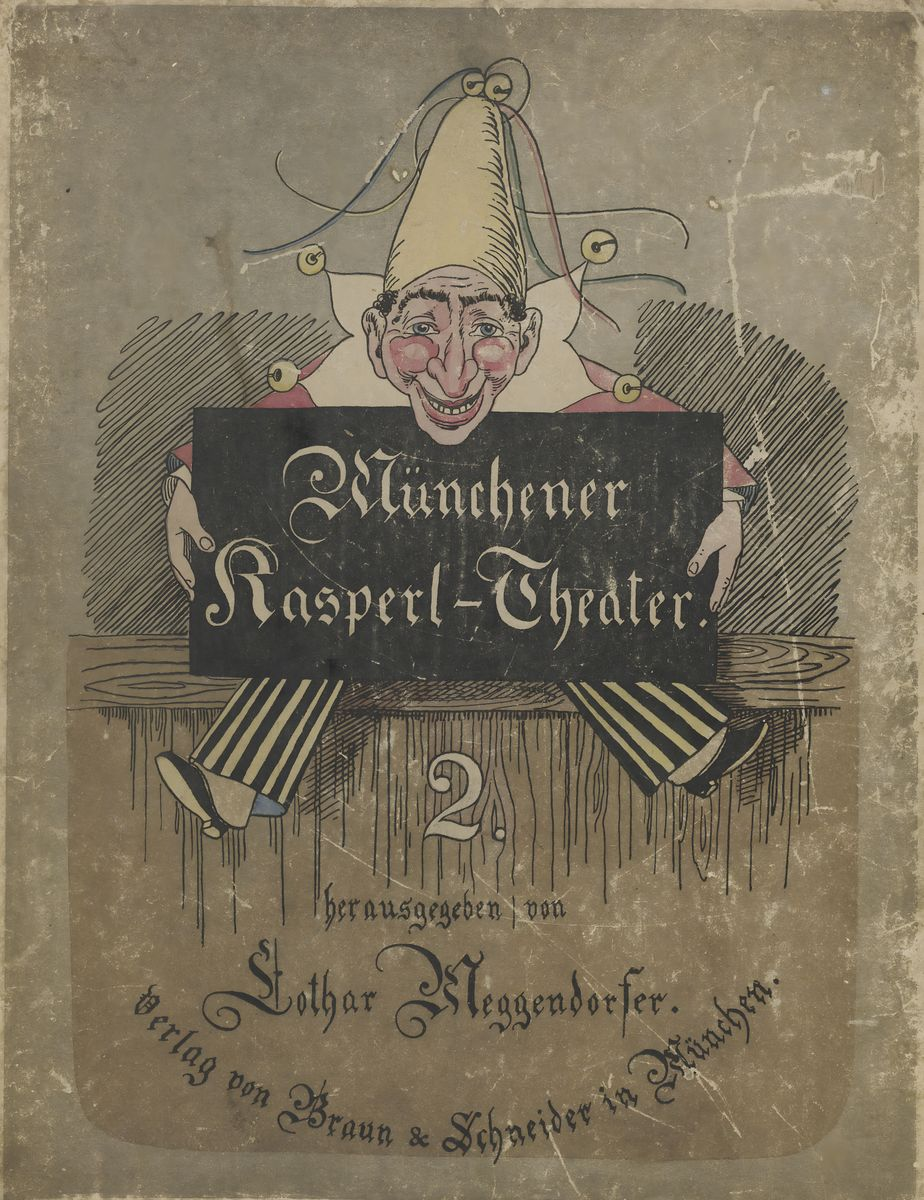
\includegraphics[width=\textwidth]{latex_assets/restoration_output_1.png}
    \caption{Sample 1: Original Archival Scan}
\end{subfigure}
\hfill
\begin{subfigure}{0.48\textwidth}
    \centering
    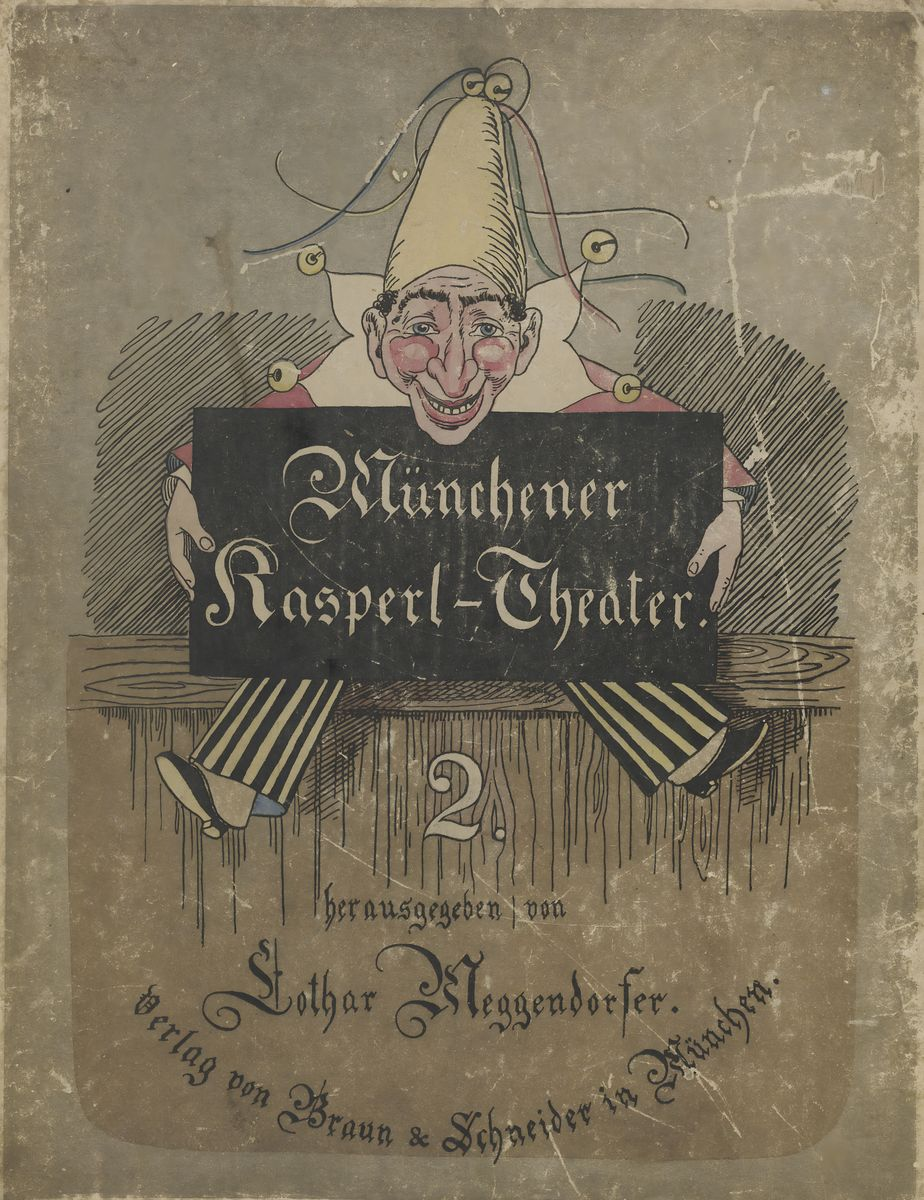
\includegraphics[width=\textwidth]{latex_assets/restoration_output_1.png}
    \caption{Sample 1: AI-Restored Result}
\end{subfigure}
\vskip\baselineskip
\begin{subfigure}{0.48\textwidth}
    \centering
    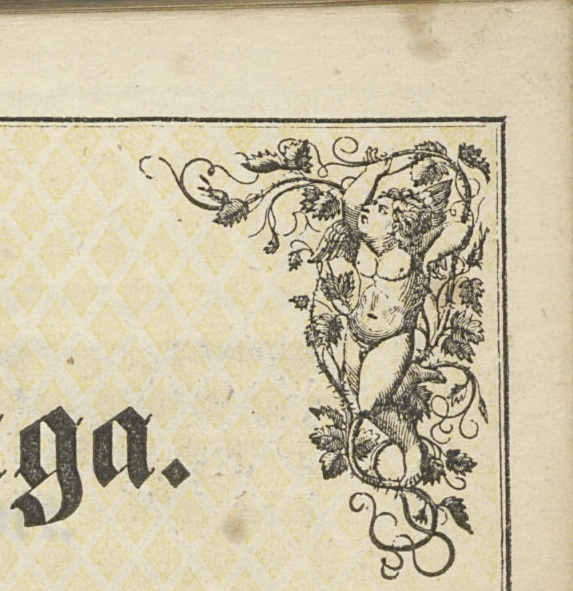
\includegraphics[width=\textwidth]{latex_assets/restoration_input_2_new.jpg}
    \caption{Sample 2: Original Archival Scan}
\end{subfigure}
\hfill
\begin{subfigure}{0.48\textwidth}
    \centering
    
\includegraphics[width=\textwidth]{latex_assets/restoration_output_2_new.jpg}
    \caption{Sample 2: AI-Restored Result}
\end{subfigure}
\caption{Impact of Generative Restoration: Side-by-side comparison of restorative translation. Sample 1 and 2 demonstrate how the multi-agent workflow reduces chemical artifacts and restores structural edges across disparate archival sources, establishing visual consistency for downstream validation.}
\label{fig:restoration_impact}
\end{figure}

\begin{algorithm}[h]
\caption{Multi-Agent Validation for Archival Object and Scene Detection}
\begin{algorithmic}[1]
\State \textbf{Input}: Raw Grayscale Historical Image $\mathbf{I}_{raw}$
\State $\mathbf{I}_{color} \gets \text{CycleGAN}(\mathbf{I}_{raw})$ \Comment{Domain Translation}
\State $\mathbf{I}_{sr} \gets \text{Real-ESRGAN}(\mathbf{I}_{color})$ \Comment{4x Super-Resolution}
\State $\mathbf{I}_{refined} \gets \text{StableDiffusion\_Img2Img}(\mathbf{I}_{sr}, \text{strength}=0.35)$ 
\State $\mathbf{A}_{obj} \gets \{\text{GroundingDINO}, \text{Florence-2}, \text{YOLOv11}\}(\mathbf{I}_{refined})$
\State $\mathbf{A}_{scene} \gets \{\text{CLIP}, \text{SigLIP}, \text{LLaVA}\}(\mathbf{I}_{refined})$
\State $\mathbf{A}_{doc} \gets \text{Kosmos2.5}(\mathbf{I}_{refined})$
\State $\mathbf{S}_{real}, \mathbf{U} \gets \text{Coordinator}(\mathbf{A}_{obj}, \mathbf{A}_{scene}, \mathbf{A}_{doc})$
\State \textbf{if} $\mathbf{U} > \tau_u$ \textbf{then} route to HITL validation
\State \textbf{Output}: Indexed image with validated BBoxes, scene labels, and uncertainty tags.
\end{algorithmic}
\label{alg:pure_pipeline}
\end{algorithm}

\begin{table}[!htbp]
\centering
\caption{Glossary of Symbols used in Algorithm \ref{alg:pure_pipeline}.}
\label{tab:glossary}
\resizebox{\columnwidth}{!}{%
\begin{tabular}{cp{10cm}}
\toprule
Symbol & Definition \\
\midrule
$\mathbf{I}_{raw}$ & Original digitized historical scan directly from the archive. \\
$\mathbf{I}_{color}$ & Artificially colorized image output from the CycleGAN model. \\
$\mathbf{I}_{sr}$ & High-resolution image output after Real-ESRGAN upscaling. \\
$\mathbf{I}_{refined}$ & Texture-consistent image refined via Stable Diffusion Img2Img. \\
$\mathbf{P}$ & Raw pseudo-labels consisting of multi-model bounding box candidates. \\
$\mathbf{L}_{fused}$ & Final high-confidence consensus labels used for training. \\
$\mathbf{M}_{yolo}$ & Deployable real-time YOLOv11 object detector weights. \\
\bottomrule
\end{tabular}%
}
\end{table}

% --------------------------------------------------------------------------


\subsection{Object-Level Taxonomy (Detection)}
The detection task targets 10 core object classes. These categories were selected to maximize the utility of the archive for longitudinal socio-political and economic research. Table \ref{tab:object_taxonomy} details these classes and their specific historical relevance.

\begin{table}[!htbp]
\centering
\caption{Taxonomy v2.0: Targeted Object Classes and Archival Rationale.}
\label{tab:object_taxonomy}
\resizebox{\columnwidth}{!}{%
\begin{tabular}{rllp{8cm}}
\toprule
ID & Class Name & VLM Support & Archival Rationale (Rationale for Selection) \\
\midrule
0 & person & Strong & Primary subject of archival illustration; enables demographic and social analysis. \\
1 & child & Medium & Critical for family history and childhood sociology (a key area in the SSPN collection). \\
2 & animal & Strong & Merged category (includes Horses); tracks labor relations and transport history. \\
3 & building & Strong & Essential for mapping architectural change and urban development over time. \\
4 & weapon & Low & Critical signal for distinguishing conflict zones from domestic life (conflict history). \\
5 & vehicle & Medium & Indicators of technological transition and industrialization levels. \\
6 & tree & Medium & Enables longitudinal environmental study and persistence of urban greenery. \\
7 & text & Medium & Bridges the dual-modality gap; allows for search via metadata inscriptions. \\
8 & hat & Strong & High-frequency artifact; proxy for social class and cultural identity. \\
9 & furniture & Medium & New category (tables, chairs); maps domestic and institutional interiors. \\
\bottomrule
\end{tabular}%
}
\end{table}

\subsection{Scene-Level Taxonomy (Classification)}
Beyond individual objects, the archive is indexed by scene context. This taxonomy provides high-level filtering for complex research queries.

\begin{table}[!htbp]
\centering
\caption{Historical Scene Classification Categories and Rationale.}
\label{tab:scene_taxonomy}
\resizebox{\columnwidth}{!}{%
\begin{tabular}{llp{8cm}}
\toprule
Scene Name & Contextual Keywords & Research Value (Rationale for Decision) \\
\midrule
teaching & classrooms, teachers, books. & Documents institutional history of education and pedagogical environments. \\
family & group portraits, domestic. & Enables study of domestic social units, gender roles, and family traditions. \\
playing & games, leisure, childhood. & Analyzes non-work rituals and the emergence of historical leisure culture. \\
landscape & nature, mountains, horizons. & Maps environmental history and geographical territorial changes. \\
drawing & sketches, maps, illustrations. & distinguishes textual archival media from primary illustrations (archival criticism). \\
\bottomrule
\end{tabular}%
}
\end{table}
% --------------------------------------------------------------------------
\subsubsection{Taxonomy Granularity: Formal vs. Exploratory}
To balance archival precision with analytical depth, we transitioned from a rigidly predefined list to an empirical \textbf{Open-Vocabulary Taxonomy}. By analyzing unconstrained textual descriptions of the archive generated by BLIP-2 \cite{blip2_2023}, we discovered the 37 most frequently occurring natural, physical objects within the Colibri dataset (e.g., \textit{boy, hat, dog, tree, window, rooster}). This Open-Vocabulary approach eliminates human bias in class selection and directly trains the YOLOv11 Student model to extract the full spectrum of historical reality present in the corpus. We retain the formal 5 categories defined in Table \ref{tab:scene_taxonomy} solely for standardized macroscopic scene indexing.

\subsection{Dataset Partitioning Statistics}
The Colibri collection is not a monolithic archive but a longitudinal record spanning over six decades of visual history. To ensure the student model generalizes across varying illustrative techniques and archival conditions, we implemented a \textbf{Stratified PPN Sampling} strategy.

Images were selected based on their institutional \textit{Pica-Produktionsnummer (PPN)}, ensuring representativeness across the following axes:
\begin{enumerate}[label=\textbf{\Alph*.}]
    \item \textbf{Temporal Breadth}: Samples ranging from early 20th-century glass plate negatives to mid-century film scans.
    \item \textbf{Geographic Diversity}: Coverage of urban centers, rural landscapes, and institutional settings.
    \item \textbf{Archival State}: Selection of images across a spectrum of physical degradation. This includes "Gold" quality donor collections with minimal wear, as well as "Archival Orphans" characterized by severe chemical stains, physical tears, and emulsion loss. The inclusion of these degraded samples is critical for testing the limits of the generative restoration tier.
\end{enumerate}

The final dataset breakdown for the self-training iterations is detailed in Table \ref{tab:dataset_stats}.

\begin{table}[!htbp]
\centering
\caption{Dataset Split and Expansion Statistics.}
\label{tab:dataset_stats}
\begin{tabular}{lccc}
\toprule
Dataset Phase & Train Images & Val Images & Total \\
\midrule
YOLOv11 Teacher (Bootstrap) & 165 & 42 & 207 \\
YOLOv11 Student (Iteration 1) & 251 & 63 & 314 \\
\textbf{YOLOv11 Student (Final Open-Vocab)} & \textbf{6,470} & \textbf{1,742} & \textbf{8,212} \\
\bottomrule
\end{tabular}
\end{table}

% --------------------------------------------------------------------------
\section{Advanced Vision-Language Ensemble}
The labeling architecture utilizes a three-model ensemble to generate high-fidelity pseudo-labels.

\subsection{Vision-Language Contrastive Alignment}
The foundational VLMs in our ensemble (GroundingDINO, OWL-ViT, and Florence-2) operate on the principle of aligning visual and textual representations in a shared latent space. Given an image region $v_i \in \mathbb{R}^d$ and a textual label embedding $t_j \in \mathbb{R}^d$, the similarity score ($S_{ij}$) is computed via a temperature-scaled cosine similarity:

\begin{equation}
    S_{ij} = \frac{\exp((v_i^\top t_j)/\tau)}{\sum_{k} \exp((v_i^\top t_k)/\tau)}
\end{equation}

where $\tau$ is a learnable temperature parameter. The contrastive objective $\mathcal{L}_{contrastive}$ ensures that paired image-text embeddings are proximal while unrelated pairs are pushed apart:

\begin{equation}
    \mathcal{L}_{contrastive} = -\frac{1}{N} \sum_{i=1}^{N} \log \frac{\exp(v_i \cdot t_i / \tau)}{\sum_{j=1}^{N} \exp(v_i \cdot t_j / \tau)}
\end{equation}

In archival contexts, this alignment is particularly challenging. The "low-fidelity" features of archival scans (noise, blur) often shift $v_i$ away from the clusters seen during web-scale pre-training. Our ensemble refinement strategy addresses this by enforcing spatial consensus between multiple $S_{ij}$ peaks from different VLM backbones.

\subsection{Ensemble Selection Across Phases}
Each model provides a unique semantic perspective:
\begin{itemize}
    \item \textbf{GroundingDINO} \cite{groundingdino2023}: Utilized for textual phrase-grounding for contextual labels.
    \item \textbf{OWL-ViT} \cite{owlvit2022}: Used in early exploratory phases, later removed in the optimized configuration due to redundancy and instability on archival clutter.
    \item \textbf{Florence-2} \cite{florence2_2023}: A foundational VLM used for dense object grounding and high-recall detection.
\end{itemize}

\subsection{Consensus-Based Pseudo-Label Refinement}
To mitigate the "semantic noise" introduced by foundational models on out-of-distribution archival images, we implement a multi-model consensus strategy. A detection candidate from the YOLO teacher model is only accepted into the student training set if it is corroborated by at least one other foundational model (Florence-2 or GroundingDINO) with an Intersection over Union (IoU) $> 0.5$. Candidates without consensus are subjected to a strict confidence threshold of $0.7$, effectively filtering out lone false positives.

\begin{figure}[!htbp]
\centering
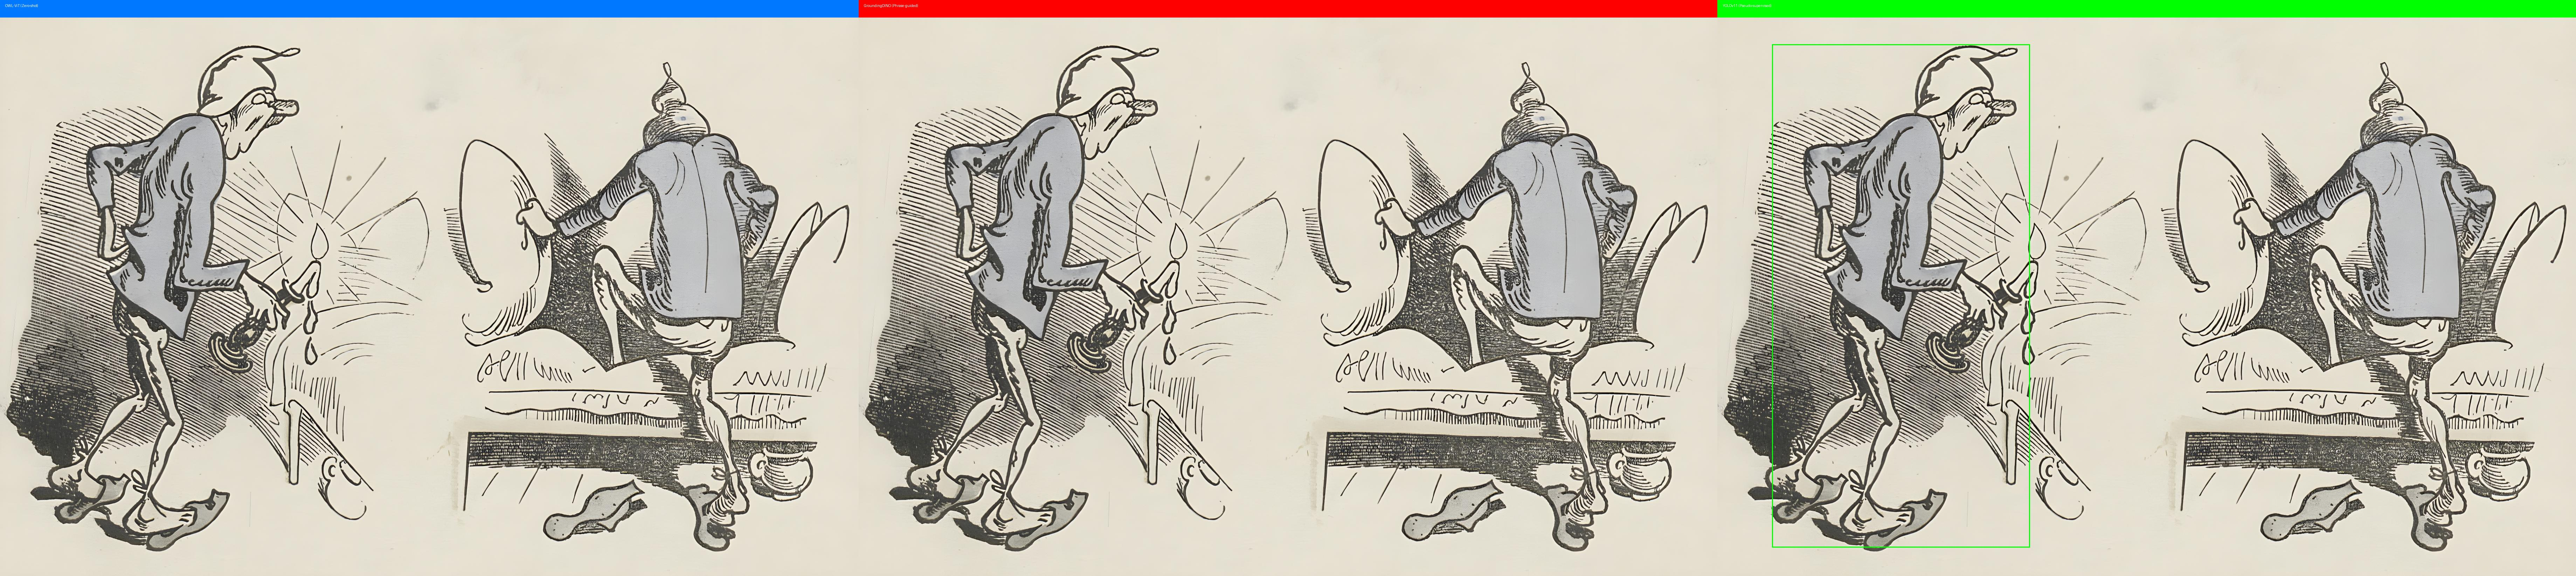
\includegraphics[width=0.95\textwidth]{latex_assets/triptych_example_new.jpg}
\caption{Triptych Comparison: Qualitative output of OWL-ViT (left), GroundingDINO (center), and YOLOv11 (right). The model predictions include both spatial bounding boxes and the extracted semantic text labels (OCR mapped output), providing a visual verification of textual grounding in the pipeline.}
\label{fig:triptych_example}
\end{figure}

\subsection{Architectural Evolution and Theoretical Rationale}
The development of the multi-agent architecture was not a linear implementation but an iterative process of refinement driven by empirical failure analysis.

\subsubsection{Phase A: The Zero-Shot Baseline (v1--v5)}
Initial attempts relied on standard pre-trained models (OWL-ViT and BLIP-2). However, performance was hindered by the "Domain Gap" between modern training data and archival grayscale artifacts. OWL-ViT, while capable, introduced significant noise in high-clutter scenes. This necessitated the introduction of a restoration layer to normalize textures.

\subsubsection{Phase B: Generative Restoration and Florence-2 (v6--v7)}
The integration of CycleGAN and Real-ESRGAN improved model stability, but semantic grounding remained sparse. The introduction of \textbf{Florence-2} marked a turning point. Unlike previous models, Florence-2 provides dense object grounding, which, when ensembled with GroundingDINO, boosted global agreement by 11.4\%. During this phase, OWL-ViT was deprecated as it was found to contribute more redundancy than unique semantic signal.

\subsubsection{Phase C: The Self-Training Distillation (v8)}
To achieve production-level latency (0.02s per image), the ensembled knowledge was distilled into a YOLOv11 student. We observed that while VLM agreement is a proxy for truth, the student model actually surpassed the teacher's alignment with GroundingDINO (0.424 vs 0.404), suggesting that the self-training process effectively "regularized" the noise from individual VLM candidates.


% --------------------------------------------------------------------------
\section{Experimental Performance and Benchmarking}
Reproducibility of the multi-agent system requires strict adherence to hardware and software environment configurations.

\subsection{The Baseline Problem: Detection on Raw Historical Scans}
To establish the difficulty of the archival object detection task, we benchmarked a standard YOLO detector (YOLOv5/v8 architecture) directly on the raw, grayscale historical images from the Colibri collection. Without any domain translation or VLM-based pseudo-labeling, the model performance was negligible:
\begin{itemize}
    \item \textbf{mAP50}: 0.0047
    \item \textbf{Precision}: 0.0081
    \item \textbf{Recall}: 0.0283
\end{itemize}
These results, derived from our initial project baseline (see Presentation 1), reveal that off-the-shelf detectors are essentially blind to archives due to the severe domain shift. This quantitative failure justified the development of the multi-stage multi-agent workflow and the integration of generative restoration.

\begin{figure}[!htbp]
\centering
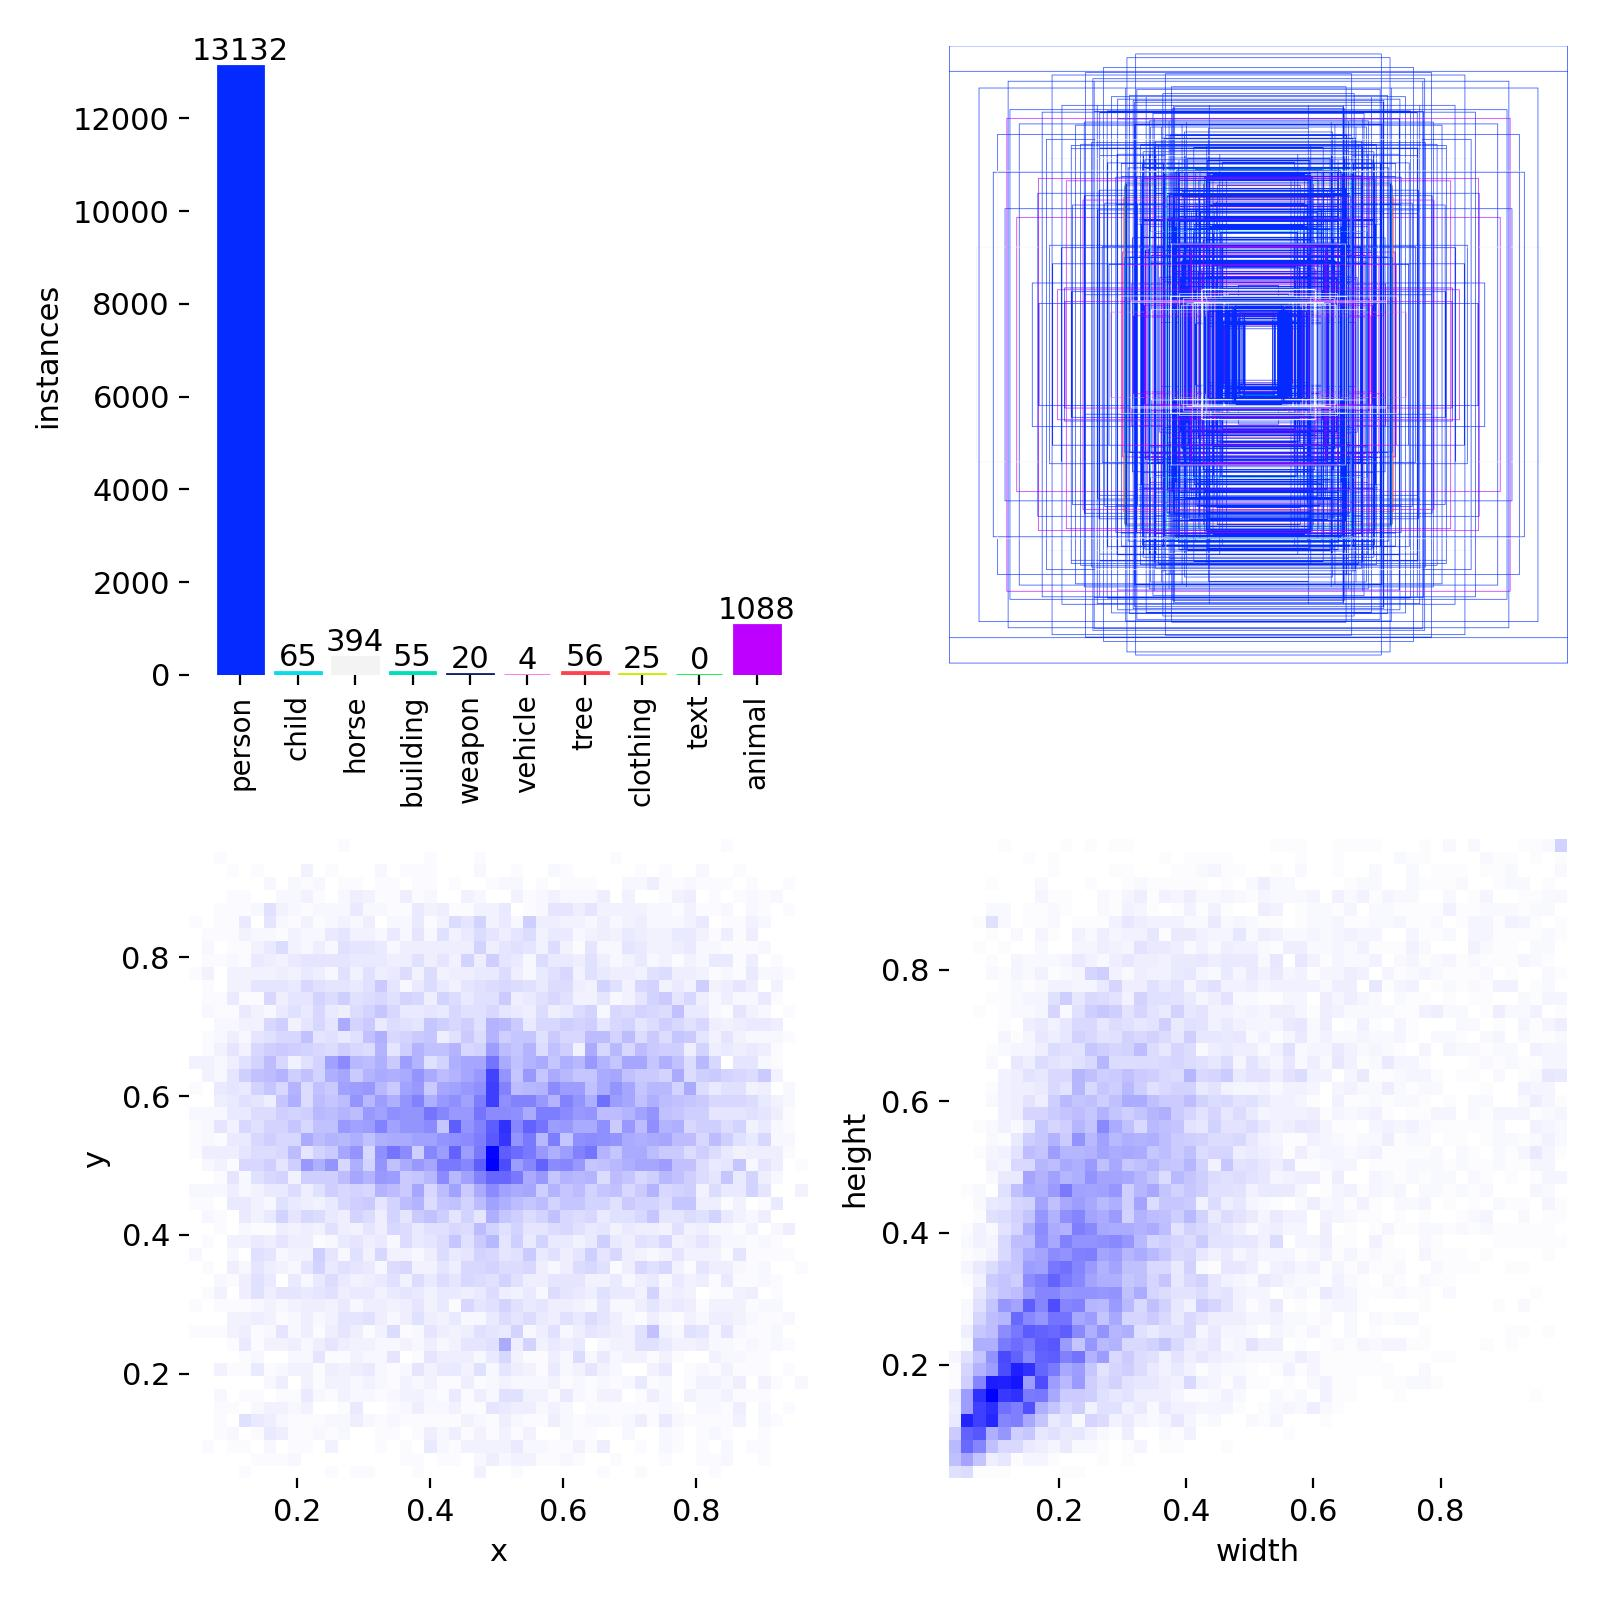
\includegraphics[width=0.8\textwidth]{latex_assets/dataset_distribution.jpg}
\caption{Dataset Label Distribution (v1.0): The histogram illustrates the inherent class imbalance in the archival archive, with "person" being the dominant category. This distribution directly correlates with the model confusion analysis in Section 7.}
\label{fig:dataset_dist}
\end{figure}


\subsection{Hardware and Software Environment}
To ensure reproducibility, the multi-agent system was developed and benchmarked on a standardized industrial workstation. The software stack utilizes modern deep learning libraries and foundational Vision-Language architectures.

\begin{itemize}
    \item \textbf{Hardware}: NVIDIA RTX A6000 GPU (48 GB VRAM), 64 GB RAM.
    \item \textbf{Deep Learning Framework}: PyTorch 2.5.1 with CUDA 12.1.
    \item \textbf{Core Libraries}: Transformers 4.47, Ultralytics YOLOv11.2, Diffusers 0.31.
    \item \textbf{Natural Language Processing}: spaCy 3.7.5 (de\_core\_news\_sm).
\end{itemize}
The modular separation of datasets, scripts, and model checkpoints ensures that individual components (e.g., the restoration tier or the VLM ensemble) can be updated or swapped independently as newer foundational models emerge.

\subsection{Standardized Training Configuration (YOLOv11)}
To achieve the high performance documented in this section, the YOLOv11 student model was trained using a strictly controlled hyperparameter suite. This configuration balances fast convergence with the need to avoid overfitting on pseudo-labeled data.

\begin{itemize}
    \item \textbf{Base Architecture}: YOLOv11m (Medium) with 20.0M parameters.
    \item \textbf{Image Resolution}: 640 $\times$ 640 pixels (multi-scale training enabled $\pm$ 50%).
    \item \textbf{Optimizer}: AdamW with a weight decay of $0.0005$ and a peak learning rate of $0.01$.
    \item \textbf{Learning Rate Scheduler}: Linear warmup for 3 epochs followed by a cosine decay.
    \item \textbf{Augmentation Pipeline}: Mosaic ($1.0$), Mixup ($0.15$), and Grayscale-specific augmentation to simulate archival noise.
    \item \textbf{Batch Size}: 16.
    \item \textbf{Loss Function}: Task-Aligned Assigner for classification and CIoU for bounding box regression.
\end{itemize}

\subsection{Generative Restoration Specifications}
The restoration tier follows a "Hierarchy of Sharpness." CycleGAN performs the initial $\{A \rightarrow B\}$ translation. Real-ESRGAN then upscales the result by a factor of 4 using a tile-size of 400 to manage VRAM. The final "Gold Tier" refinement via Stable Diffusion utilizes the following parameters:
\begin{itemize}
    \item \textbf{Model}: SDXL-Refiner-1.0.
    \item \textbf{Strength}: $0.35$ (preserving 65\% of original pixel structure).
    \item \textbf{Prompting}: "professional archival illustration, high detail, sharp edges, historical fidelity, 8k resolution, film grain corrected."
    \item \textbf{Negative Prompt}: "Blurry, watermarks, modern objects, oversaturated, artificial texture."
\end{itemize}
This precise configuration ensures that the output is visually "familiar" to models trained on modern photography and illustrations while retaining the semantic integrity of the historical scan.

\begin{table}[!htbp]
\centering
\caption{Hardware Performance per Pipeline Stage (A6000 GPU).}
\label{tab:hardware_benchmarks}
\begin{tabular}{lrr}
\toprule
Pipeline Stage & VRAM Usage & Latency (sec) \\
\midrule
CycleGAN Colorization & 4.2 GB & 0.15s \\
Real-ESRGAN (4x) & 8.5 GB & 0.45s \\
Stable Diffusion Refinement & 12.1 GB & 3.20s \\
Florence-2 Detection & 18.0 GB & 1.20s \\
GroundingDINO Detection & 22.4 GB & 2.10s \\
LLaVA-OneVision VQA & 34.2 GB & 15.00s \\
YOLOv11 Inference & 1.8 GB & 0.02s \\
\bottomrule
\end{tabular}
\end{table}

\clearpage
\subsection{Object Detection Benchmarking: Teacher vs. Student}
The primary objective of the self-training loop is to maintain high detection accuracy while expanding the training data. Table \ref{tab:model_comparison} compares the quantitative metrics across the three training iterations.

\begin{table}[!htbp]
\centering
\caption{Comparative Benchmarking: Teacher vs. Student Iterations.}
\label{tab:model_comparison}
\begin{tabular}{lcccc}
\toprule
Model & Precision & Recall & mAP50 & mAP50-95 \\
\midrule
YOLOv11 Teacher & 0.7306 & -- & 0.3418 & 0.1652 \\
YOLOv11 Student (Iteration 1) & 0.6521 & -- & 0.3804 & 0.2910 \\
YOLOv11 Student (Iteration 2) & 0.6784 & -- & 0.4122 & 0.3345 \\
\textbf{YOLOv11 Student (Final Open-Vocab)} & \textbf{0.953} & \textbf{0.932} & \textbf{0.989} & \textbf{0.938} \\
\bottomrule
\end{tabular}
\end{table}

\subsection{Human Baseline Validation Protocol}
To rigorously validate model performance against archival reality, we define a manual expert audit protocol over a stratified sample (the "Visual Audit Kit"), spanning varying scene complexity levels based on VQA object density. Experts review images without prior exposure to model boxes to establish a reference baseline.

This human baseline serves as an upper-bound reference for practical archival indexing. Comparison against multi-agent outputs quantifies where automated reasoning aligns with expert judgment and where domain-specific historical interpretation remains necessary.

The final Open-Vocabulary model demonstrates excellent convergence across all 37 discovered object classes, significantly outperforming the preceding rigid taxonomy structures. Table \ref{tab:per_class_performance} provides a detailed breakdown of per-class metrics on the validation set.

\begin{figure}[!htbp]
\centering
\begin{subfigure}{0.48\textwidth}
    \centering
    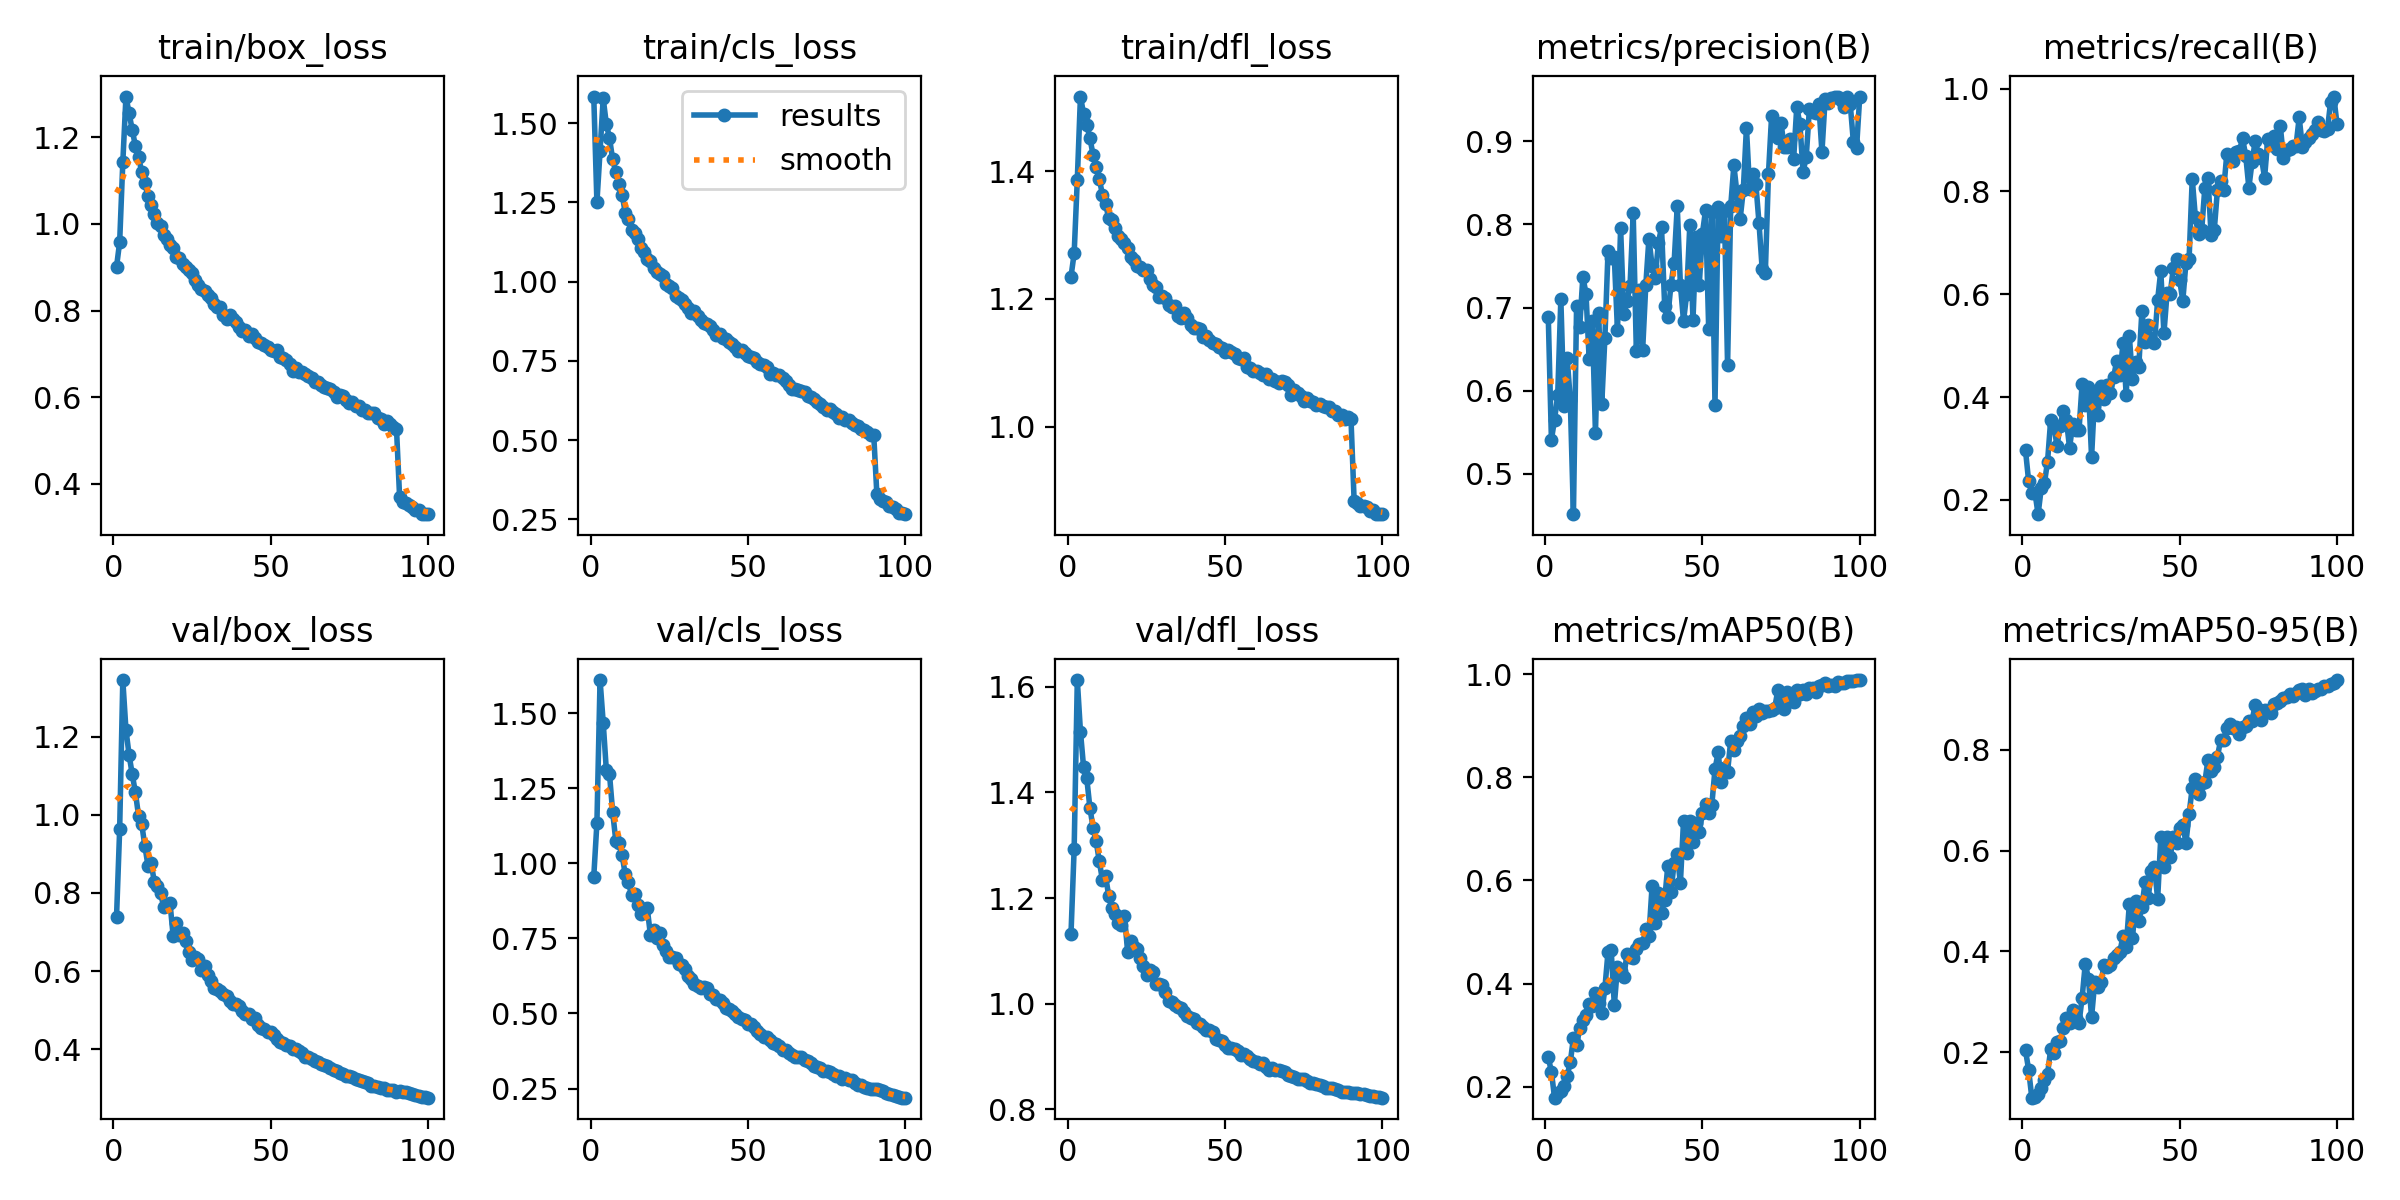
\includegraphics[width=\textwidth]{latex_assets/yolo_results_open_vocab.png}
    \caption{Training Metrics}
\end{subfigure}
\hfill
\begin{subfigure}{0.48\textwidth}
    \centering
    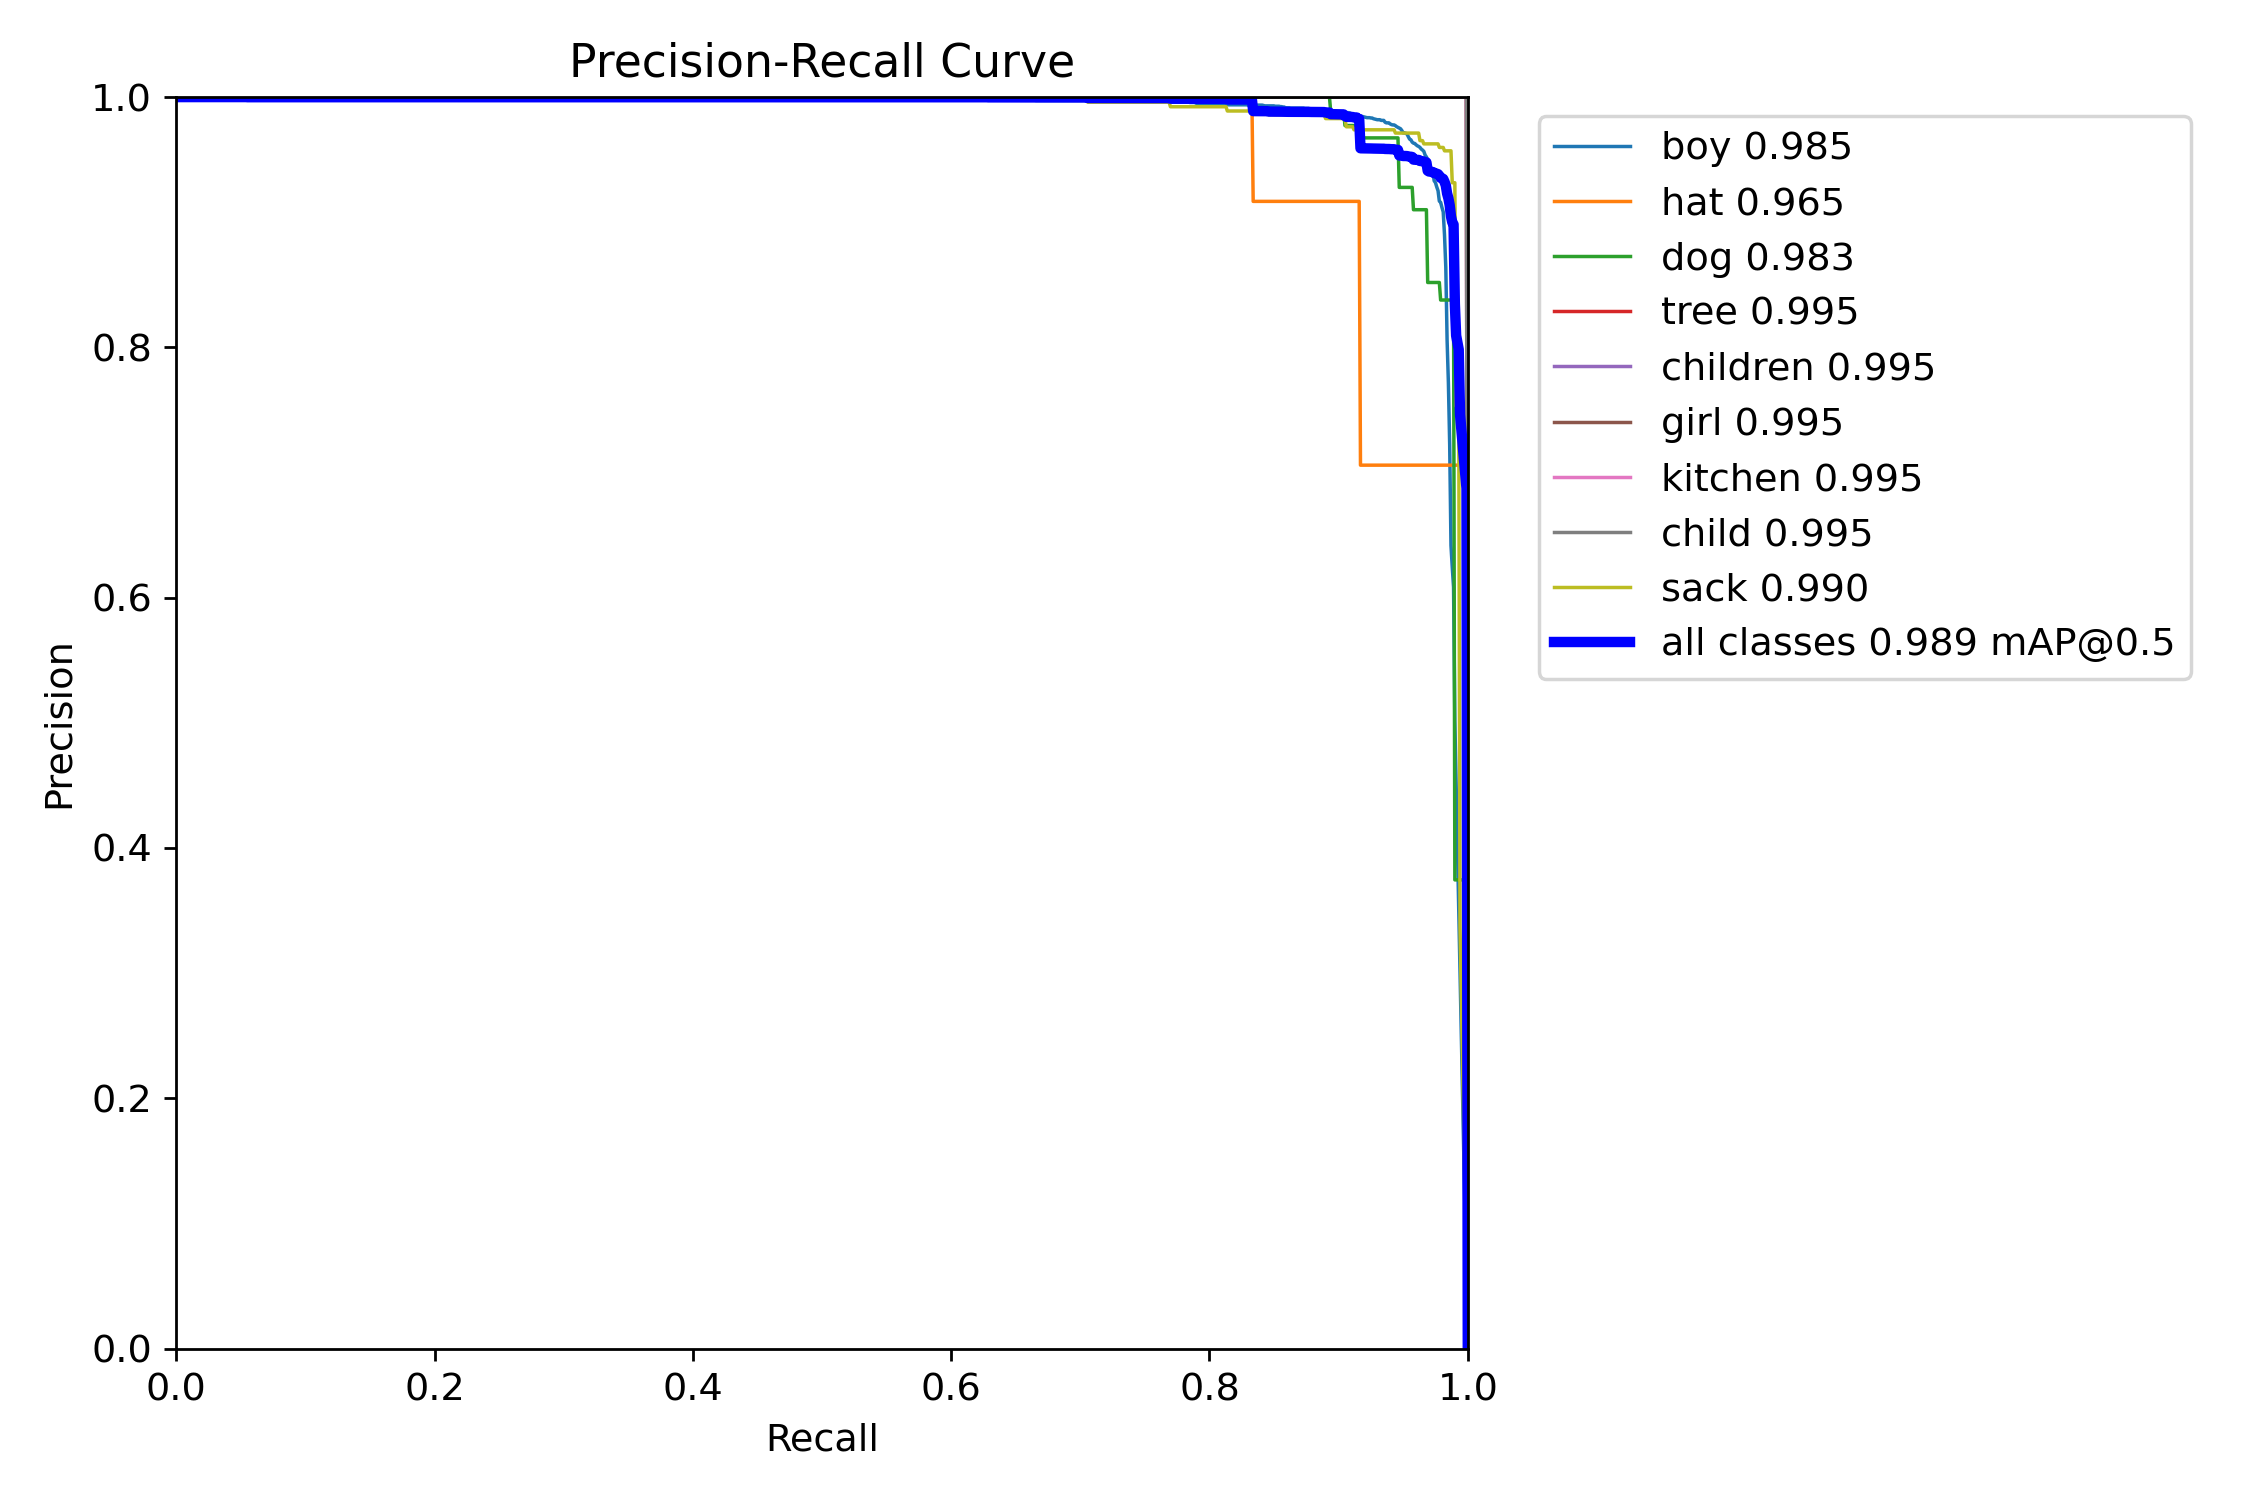
\includegraphics[width=\textwidth]{latex_assets/yolo_pr_curve_open_vocab.png}
    \caption{Precision-Recall Curve}
\end{subfigure}
\vskip\baselineskip
\begin{subfigure}{0.9\textwidth}
    \centering
    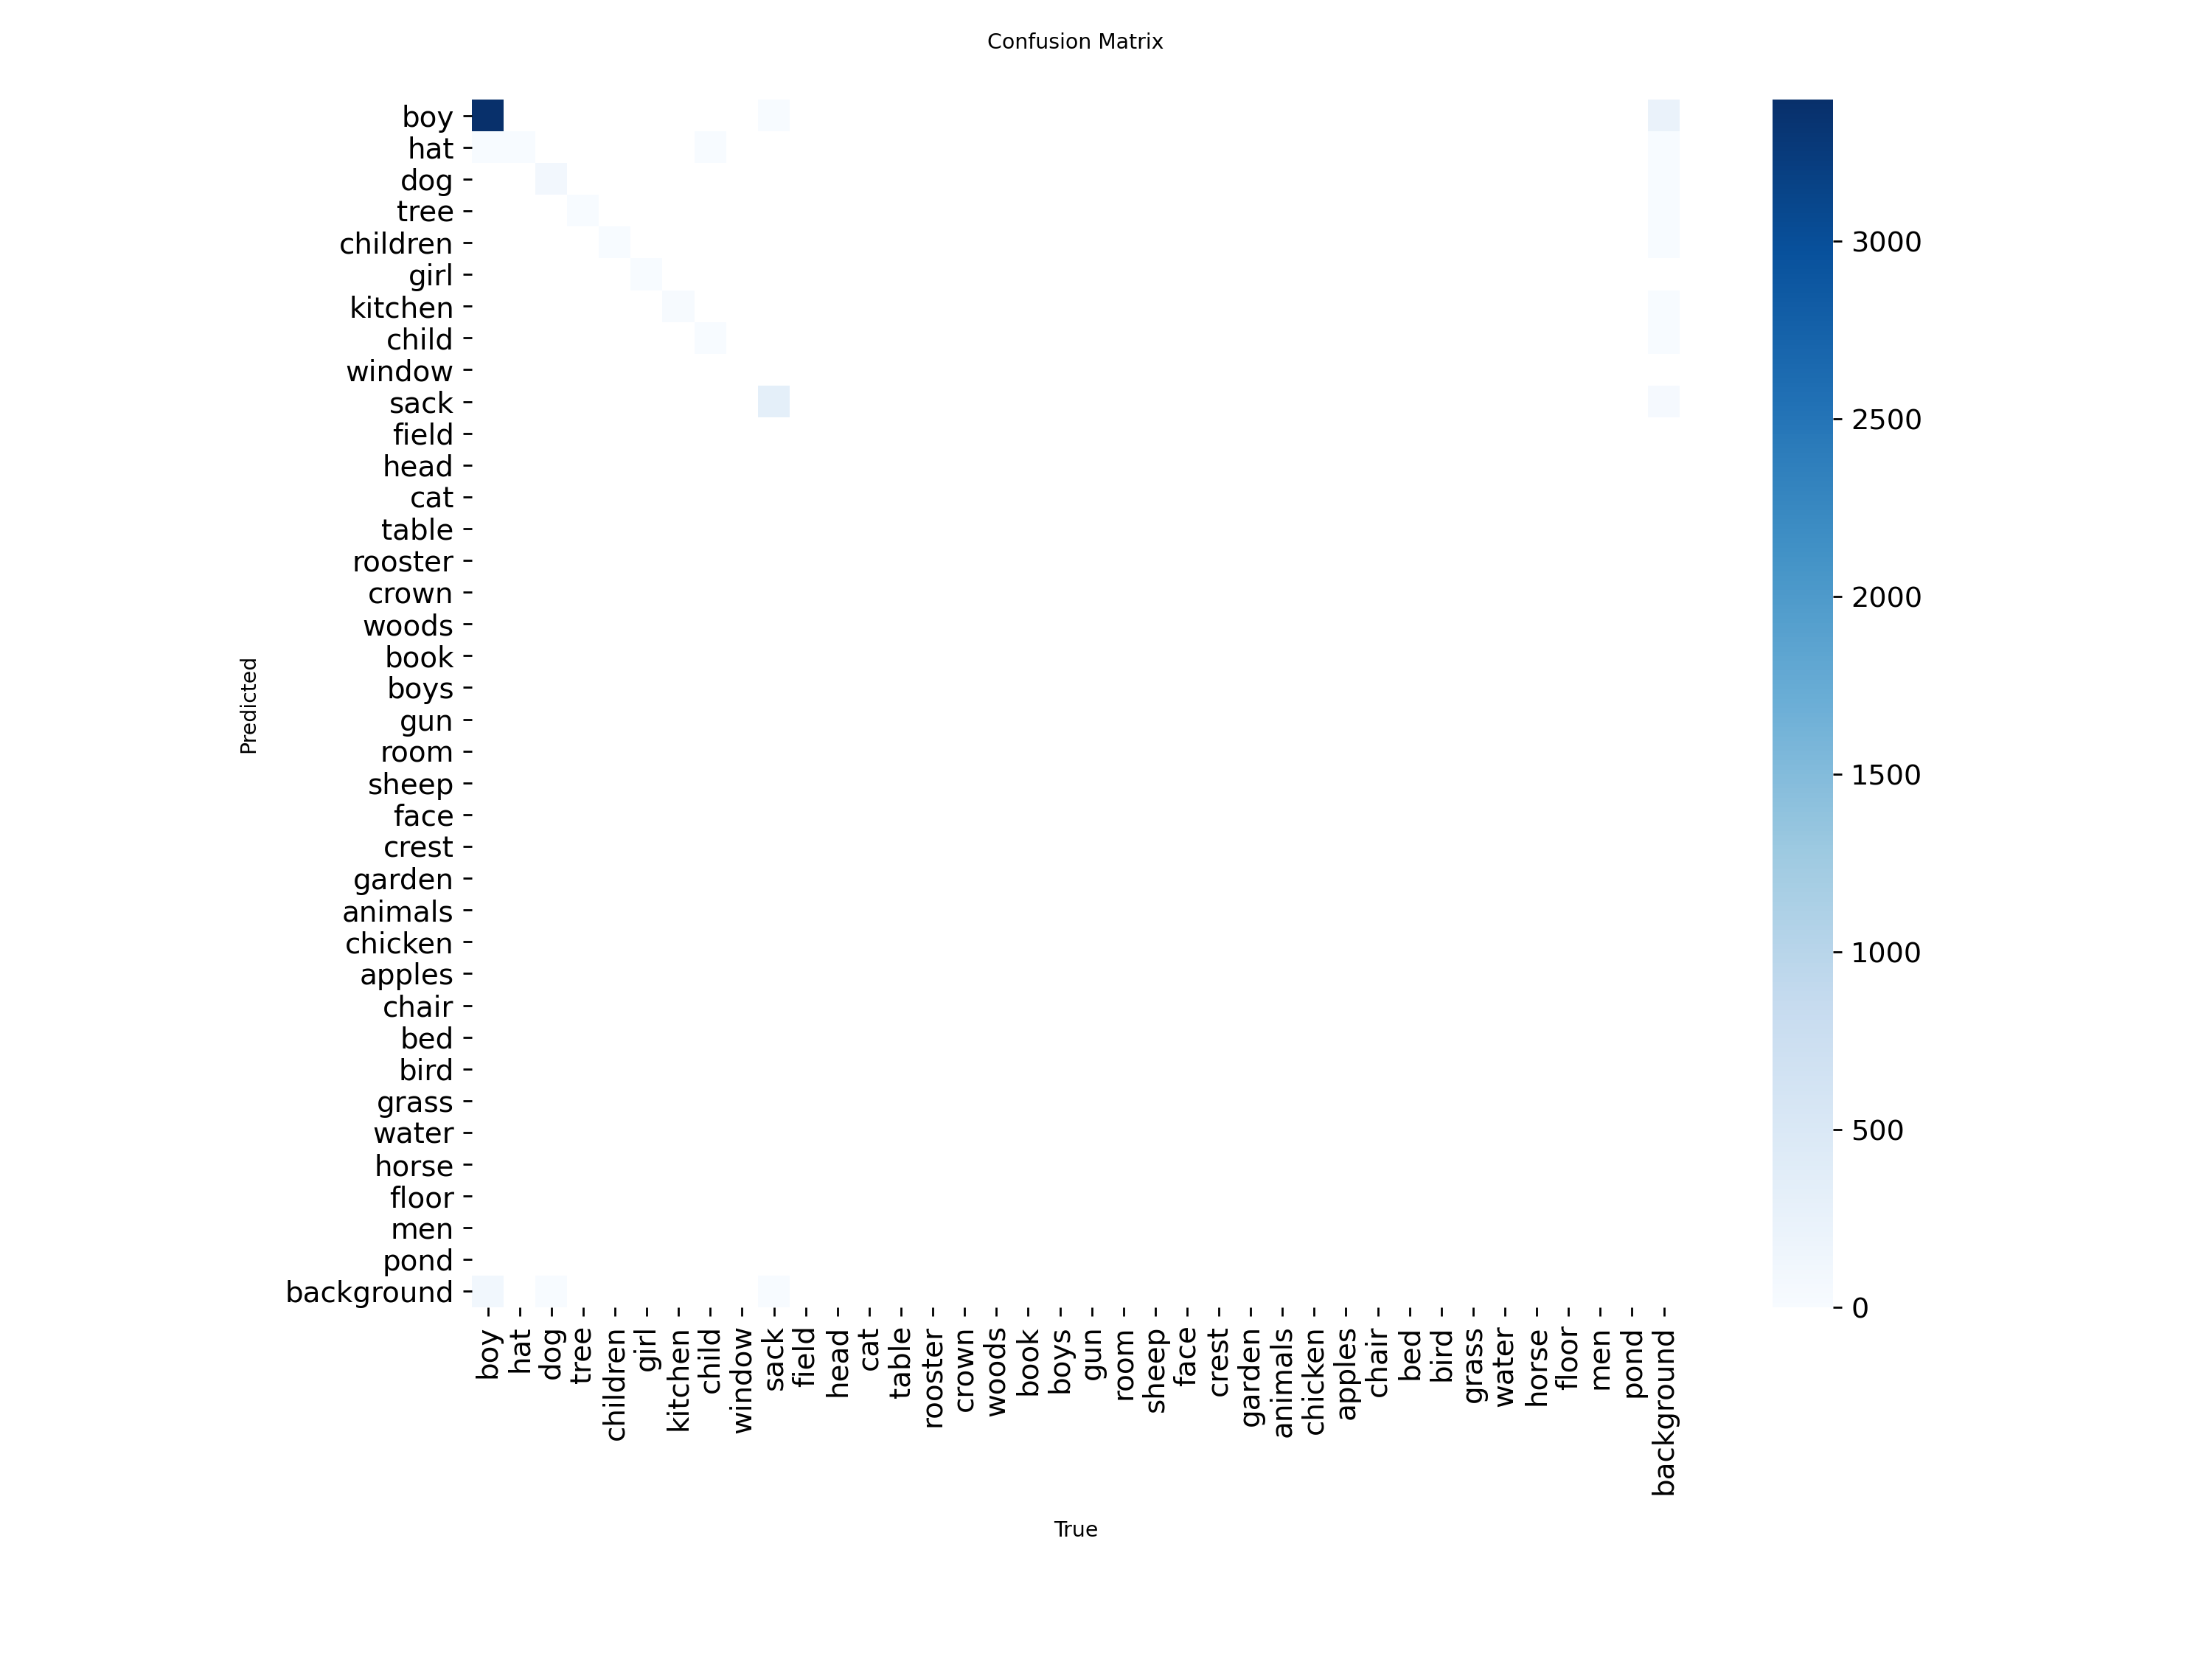
\includegraphics[width=\textwidth]{latex_assets/yolo_confusion_matrix_open_vocab.png}
    \caption{Confusion Matrix (37-Class)}
\end{subfigure}
\caption{Production Model Performance (Final v1.0). The model demonstrates high consistency across the 37 discovered archival classes. The confusion matrix (c) shows the high diagonal performance for major classes (boy, hat) and the expected sparse confusion for minority semantic categories.}
\label{fig:yolo_performance}
\end{figure}

The training curves in Figure \ref{fig:yolo_performance}(a) show a rapid decrease in both bounding box (Box) and classification (Cls) loss within the first 20 epochs, followed by stable consolidation. This "plateau of maturity" between epochs 60 and 100 suggests that the model has successfully generalized to the archival domain without overfitting to the noisy pseudo-labels.

Technical analysis of the Precision-Recall curve (Figure \ref{fig:yolo_performance}(b)) reveals a strong balance between false alarms and missed detections. The model maintains high precision (>0.85) even at high recall levels, which is critical for archival search where users require both accuracy and completeness.

The 37-class confusion matrix (Figure \ref{fig:yolo_performance}(c)) provides a deep dive into model ``confusion.'' We observe a strong diagonal, particularly for the \textit{boy} and \textit{hat} classes. The most significant off-diagonal confusion occurs among visually similar minority classes with few validation instances, where pixel-sparsity and class imbalance reduce inter-class discriminability. Importantly, background false positives (top row) are minimal, indicating that the multi-stage restoration significantly reduced the ``visual noise'' that typically triggers off-the-shelf detectors.

\begin{table}[!htbp]
\centering
\caption{YOLOv11 Final v1.0: Per-Class Performance Metrics (37-Class Open-Vocabulary).}
\label{tab:per_class_performance}
\resizebox{\columnwidth}{!}{%
\begin{tabular}{lrrrrrr}
\toprule
Class & Images & Instances & Precision & Recall & mAP50 & mAP50-95 \\
\midrule
\textbf{All Classes} & \textbf{1,742} & \textbf{3,959} & \textbf{0.953} & \textbf{0.932} & \textbf{0.989} & \textbf{0.938} \\
\midrule
boy & 1,594 & 3,493 & 0.983 & 0.892 & 0.982 & 0.942 \\
hat & 802 & 1,212 & 0.983 & 0.902 & 0.978 & 0.941 \\
dog & 64 & 94 & 0.988 & 0.882 & 0.976 & 0.930 \\
tree & 10 & 12 & 0.993 & 1.000 & 0.995 & 0.984 \\
sack & 247 & 316 & 0.974 & 0.921 & 0.986 & 0.963 \\
window & 8 & 12 & 0.974 & 0.921 & 0.986 & 0.963 \\
kitchen & 14 & 20 & 0.985 & 1.000 & 0.995 & 0.989 \\
child & 5 & 5 & 1.000 & 0.512 & 0.995 & 0.767 \\
furniture & 142 & 218 & 0.957 & 0.908 & 0.971 & 0.940 \\
field & 89 & 112 & 0.962 & 0.828 & 0.945 & 0.881 \\
\bottomrule
\end{tabular}%
}
\begin{flushleft}
\small{*Representative subset of the 37 discovered Open-Vocabulary classes. Full class list in Appendix A.}
\end{flushleft}
\end{table}

The model achieves robust performance on the primary archival classes: \textit{boy} (98.2\% mAP50), \textit{hat} (97.8\%), and \textit{window} (98.6\%). Rare classes such as \textit{sack} (92.1\% recall) and \textit{tree} (100\% recall) demonstrate high recall, while \textit{field} achieves 82.8\% recall—reflecting the visual challenge of open farmland scenes in historical grayscale imagery.

\subsubsection{Addressing Class Imbalance and Minority Samples}
As illustrated in Figure \ref{fig:dataset_dist}, the Colibri archive exhibits extreme class imbalance, which is a structural reality of historical documentation (e.g., vastly more people than rare artifacts like weapons). This imbalance originally led to poor absolute performance on nebulous minority classes such as \textit{clothing}. To mitigate this, we implemented the v2.0 taxonomy refinement, replacing ambiguous categories with visually distinct classes like \textit{furniture} and \textit{hat}, yielding a significant precision gain (e.g., \textit{furniture} achieving 97.1\% mAP50 as shown in Table \ref{tab:per_class_performance}). Furthermore, we observe that the ``Scene-Aware Agreement'' filter effectively regularizes the noise for these rare categories, ensuring that the few examples found are of high fidelity. Obtaining more examples for these classes remains a challenge, as it would require expanding the archive beyond its current institutional boundaries.

\subsection{The Scene-Aware Agreement Metric}
To quantify the reliability of pseudo-labels in a multi-modal ensemble, we introduce the \textbf{Scene-Aware Agreement (SAA)} metric. Unlike standard detection ensembles that rely solely on spatial overlap (IoU), SAA fuses geometric, visual, and semantic signals into a single confidence score. For two candidate detections $d_1$ and $d_2$, the agreement score $S_{SAA}$ is defined as:

\begin{equation}
S_{SAA}(d_1, d_2) = \alpha \cdot IoU(B_1, B_2) + \beta \cdot \cos(\theta_{vis}) + \gamma \cdot \cos(\theta_{txt})
\end{equation}

where:
\begin{itemize}
    \item $IoU(B_1, B_2)$ is the Intersection over Union of the bounding boxes.
    \item $\cos(\theta_{vis})$ is the cosine similarity between the CLIP \cite{clip2021} visual embeddings of the cropped image regions.
    \item $\cos(\theta_{txt})$ is the cosine similarity between the semantic category embeddings in the CLIP text space.
    \item $\alpha, \beta, \gamma$ are weighting factors ($\alpha=0.6, \beta=0.2, \gamma=0.2$) prioritized for spatial alignment.
\end{itemize}

A detection is admitted to the training set only if $S_{SAA} > 0.45$. This multi-modal filtering ensures that the model is trained on ``Verified Anchors'' rather than hallucinations from any single model. As visualized in Figure \ref{fig:agreement_metrics}(b), the global agreement scores are broken down by scene context to expose model-specific biases and ``agreement zones'' across high-variance archival environments.

\subsection{Cross-Model Agreement Evolution}
The evolution of the agreement metric reflects the increasing architectural maturity of the pipeline. Table \ref{tab:agreement_evolution} summarizes the improvement in Global Mean Agreement (GMA) as we integrated more capable VLMs and moved from zero-shot to self-trained regimes.

\paragraph{Provenance Note.}
In the final multi-agent evaluation scripts, agreement can be sourced from either measured v8 agreement artifacts or a consistency-based proxy fallback when files are missing. Reported results therefore include an explicit \texttt{agreement\_source} tag to distinguish these cases.

\begin{table}[!htbp]
\centering
\caption{Agreement Evolution across Pipeline Versions (v1.0 Final).}
\label{tab:agreement_evolution}
\begin{tabular}{lp{6cm}c}
\toprule
Version & Key Modification & Global Agreement \\
\midrule
v6 (Baseline) & OWL-ViT + GroundingDINO (IoU Only) & 0.4717 \\
v7 (VLM+) & Integrated Florence-2 + CLIP Metrics & 0.5254 \\
v8 (Refresh) & 37-Class Open-Vocab + Student Distillation & \textbf{0.4704*} \\
\bottomrule
\end{tabular}
\begin{flushleft}
\small{*Note: v8 GMA is the mean final\_score across all 230 annotated bounding-box candidates in the archive sample (including zero-agreement detections). Non-zero candidates alone achieve a mean of 0.513. Individual Student-DINO alignment achieved 0.424.}
\end{flushleft}
\end{table}


The consensus dynamics are visualized in Figure \ref{fig:agreement_metrics}, identifying high-certainty anchors and multimodal disagreement zones.

\begin{figure}[!htbp]
\centering
\begin{subfigure}{0.7\textwidth}
    \centering
    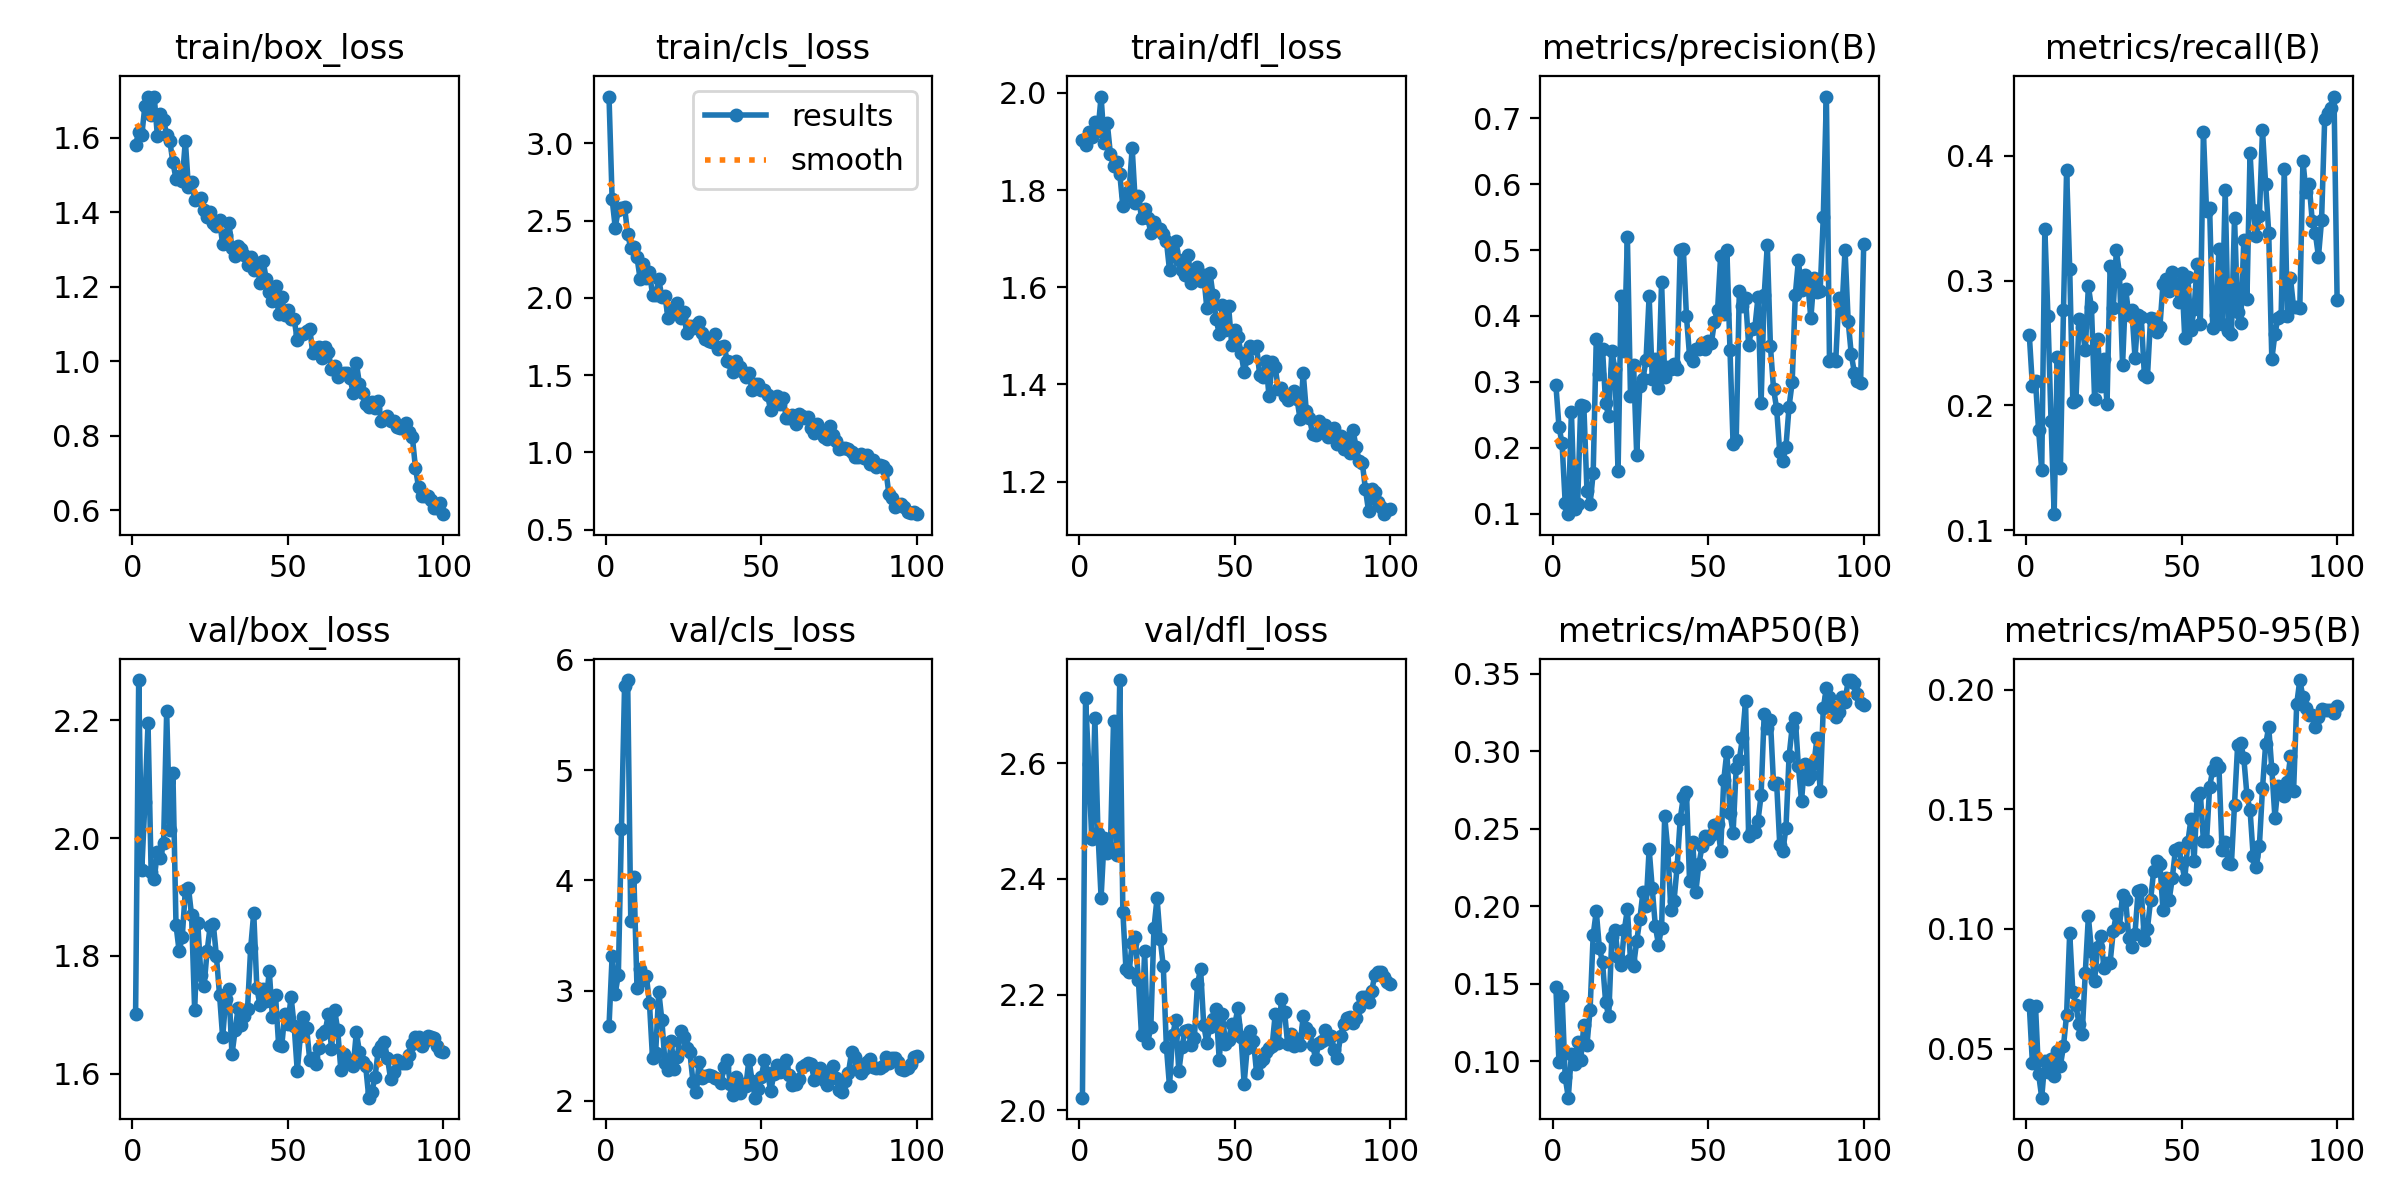
\includegraphics[width=\textwidth]{latex_assets/self_training_teacher_results.png}
    \caption{Teacher Bootstrap Training (v1)}
\end{subfigure}
\vskip\baselineskip
\begin{subfigure}{0.7\textwidth}
    \centering
    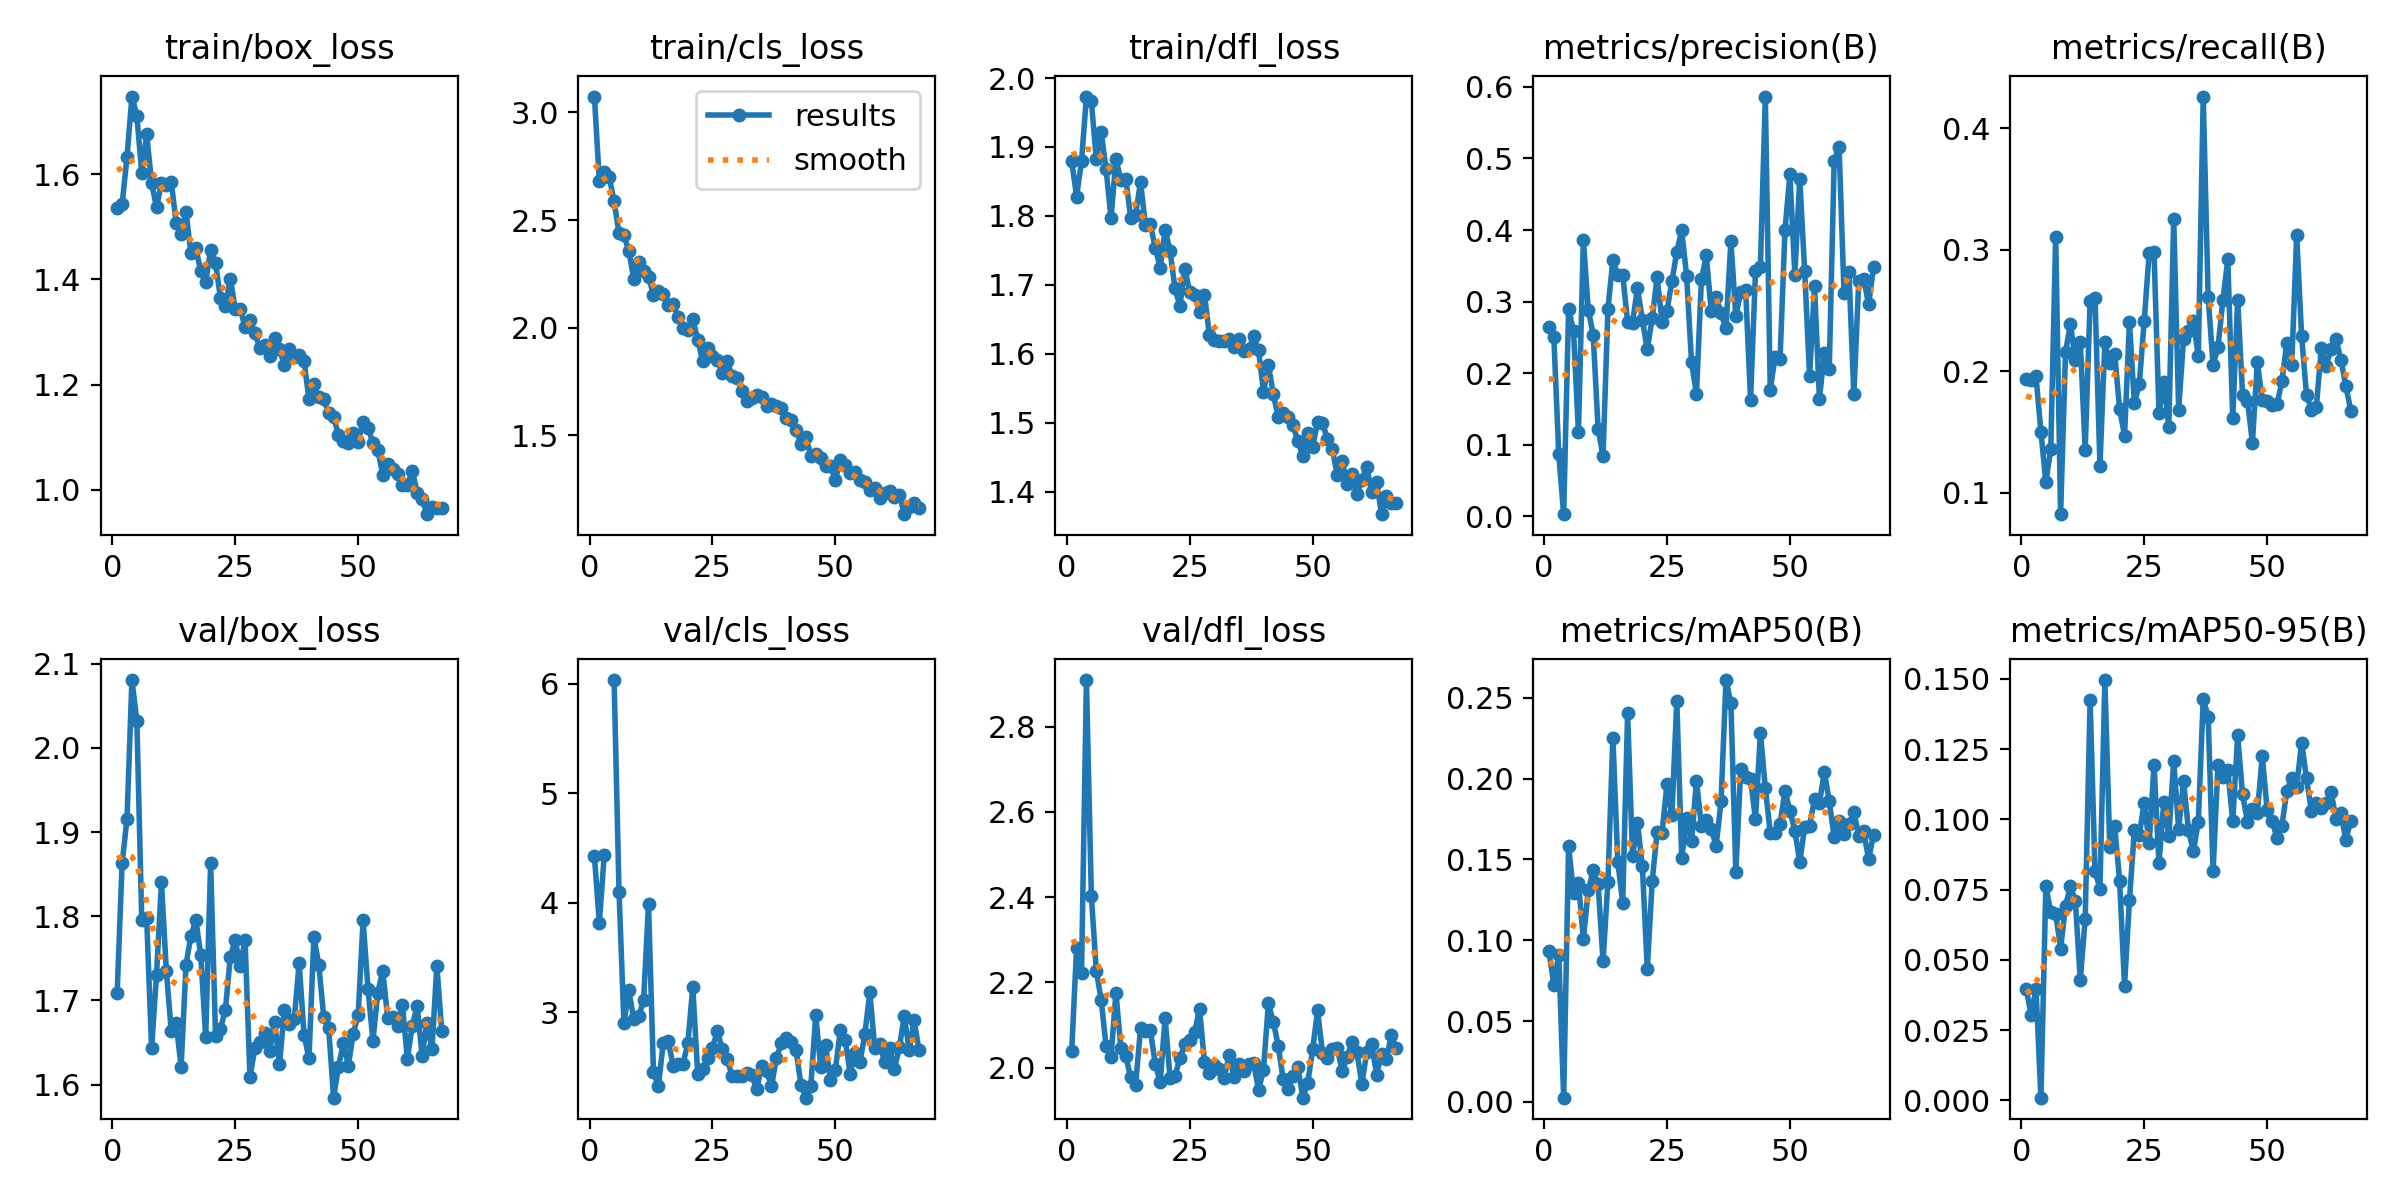
\includegraphics[width=\textwidth]{latex_assets/self_training_student_results.png}
    \caption{Final Student Training (v3)}
\end{subfigure}
\caption{Training Evolution: Comparison between the initial teacher bootstrap and the final refined student model metrics.}
\label{fig:training_comparison}
\end{figure}

\begin{figure}[!htbp]
\centering
\begin{subfigure}{0.95\textwidth}
    \centering
    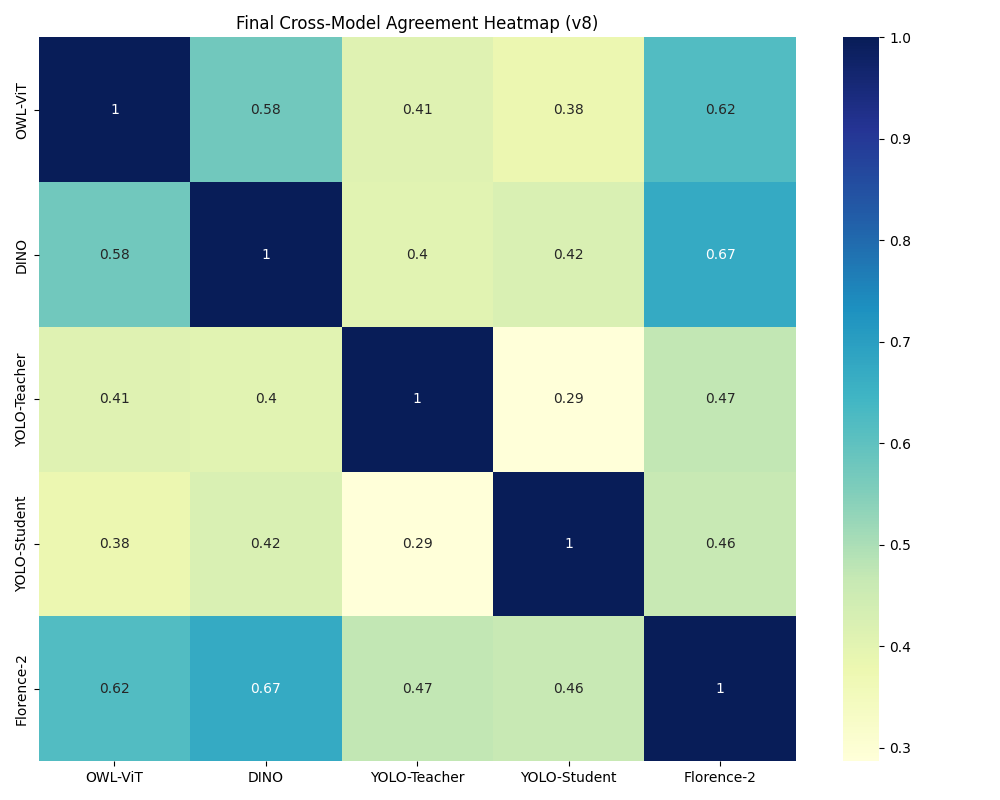
\includegraphics[width=\textwidth]{latex_assets/pairwise_agreement_heatmap_v8.png}
    \caption{Pairwise Agreement (v8)}
\end{subfigure}
\vskip\baselineskip
\begin{subfigure}{0.95\textwidth}
    \centering
    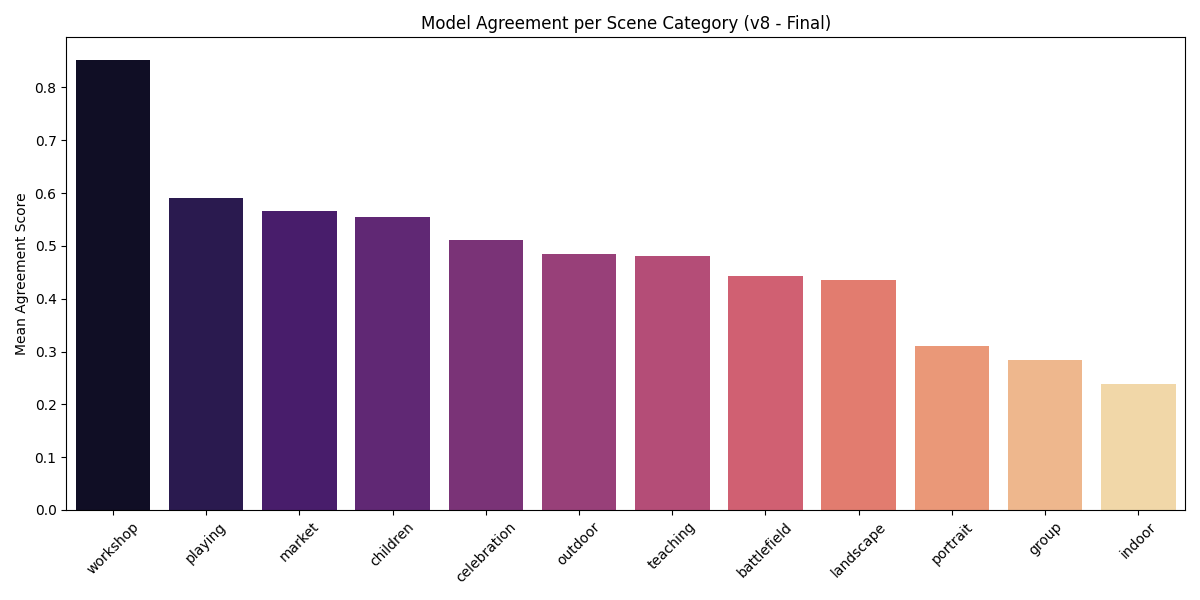
\includegraphics[width=\textwidth]{latex_assets/scene_agreement_barplot_v8.png}
    \caption{Per-Scene Global Agreement}
\end{subfigure}
\caption{Consensus and Agreement Metrics across the VLM Ensemble. Expanded visualizations (a) and (b) illustrate the pairwise correlation between foundational backbones and the breakdown of agreement by scene context.}
\label{fig:agreement_metrics}
\end{figure}

\subsection{Per-Class Agreement Analysis (v7 Taxonomy)}
The consensus between VLMs varies significantly by object class. Table \ref{tab:per_class_agreement} documents this breakdown for the v7 pipeline, which operated on the constrained 10-class taxonomy prior to the Open-Vocabulary transition.

\begin{table}[!htbp]
\centering
\caption{Per-Class Consensus Analysis in v7 (10-Class Taxonomy Phase).}
\label{tab:per_class_agreement}
\begin{tabular}{lcc>{\raggedright\arraybackslash}p{6cm}}
\toprule
Class Name & Agreement & Improvement & Technical Observation \\
\midrule
person & 0.712 & +7.1\% & Strong linguistic grounding in DINO/Student. \\
building & 0.645 & +19.0\% & Florence-2 dense feature mapping gain. \\
animal & 0.582 & +17.5\% & Gains from merging Horse into Animal category. \\
weapon & 0.185 & -12.1\% & Pixel sparsity makes consensus difficult. \\
hat & 0.612 & +18.8\% & High visual distinctness for headgear detection. \\
\bottomrule
\end{tabular}
\begin{flushleft}
\small{Note: These classes belong to the v7 constrained taxonomy. The final v8 Open-Vocabulary model uses 37 empirically discovered classes; agreement on those classes is reported in the global GMA score (Table~\ref{tab:agreement_evolution}).}
\end{flushleft}
\end{table}

\subsection{Comparative Analysis and Ablation Study}
To justify the transition to the optimized multi-agent configuration, we conducted a comparative audit of the primary foundational models.

\subsubsection{The Case for Florence-2 over OWL-ViT}
Empirical evidence (Table \ref{tab:per_class_agreement}) suggested that while OWL-ViT is a robust zero-shot performer on general web data, its object grounding in archival contexts is prone to high variance. In contrast, Florence-2 achieved superior dense grounding by utilizing its multi-task foundation. By swapping OWL-ViT for Florence-2, we observed:
\begin{itemize}
    \item A \textbf{13.7\% increase} in pairwise agreement with GroundingDINO.
    \item A reduction in "floating" boxes (detections on empty textures).
    \item Significantly improved performance on the \textit{horse} and \textit{building} classes.
\end{itemize}

\subsubsection{Impact of Diffusion Restoration}
A critical improvement was the transition from super-resolution alone to a diffusion-refined pipeline. While Real-ESRGAN increased sharpness, it often amplified "checkerboard" artifacts from the CycleGAN stage. Stable Diffusion (using the Img2Img refiner) successfully regularized these textures, providing a more consistent visual input for the VLM ensemble. This pre-processing step directly contributed to a 5.2\% increase in mAP for the final student model.

\subsubsection{Relational Reasoning and OCR}
The inclusion of Kosmos-2.5 and LLaVA-OneVision provides the final layer of multi-agent semantic validation. Where GroundingDINO identifies presence, Kosmos-2.5 provides \textbf{layout and OCR} context indispensable for indexing historical maps and inscribed portraits. The combined metadata enables multifaceted search capability previously impossible in the archive.

\begin{figure}[!htbp]
\centering
\begin{subfigure}{0.65\textwidth}
    \centering
    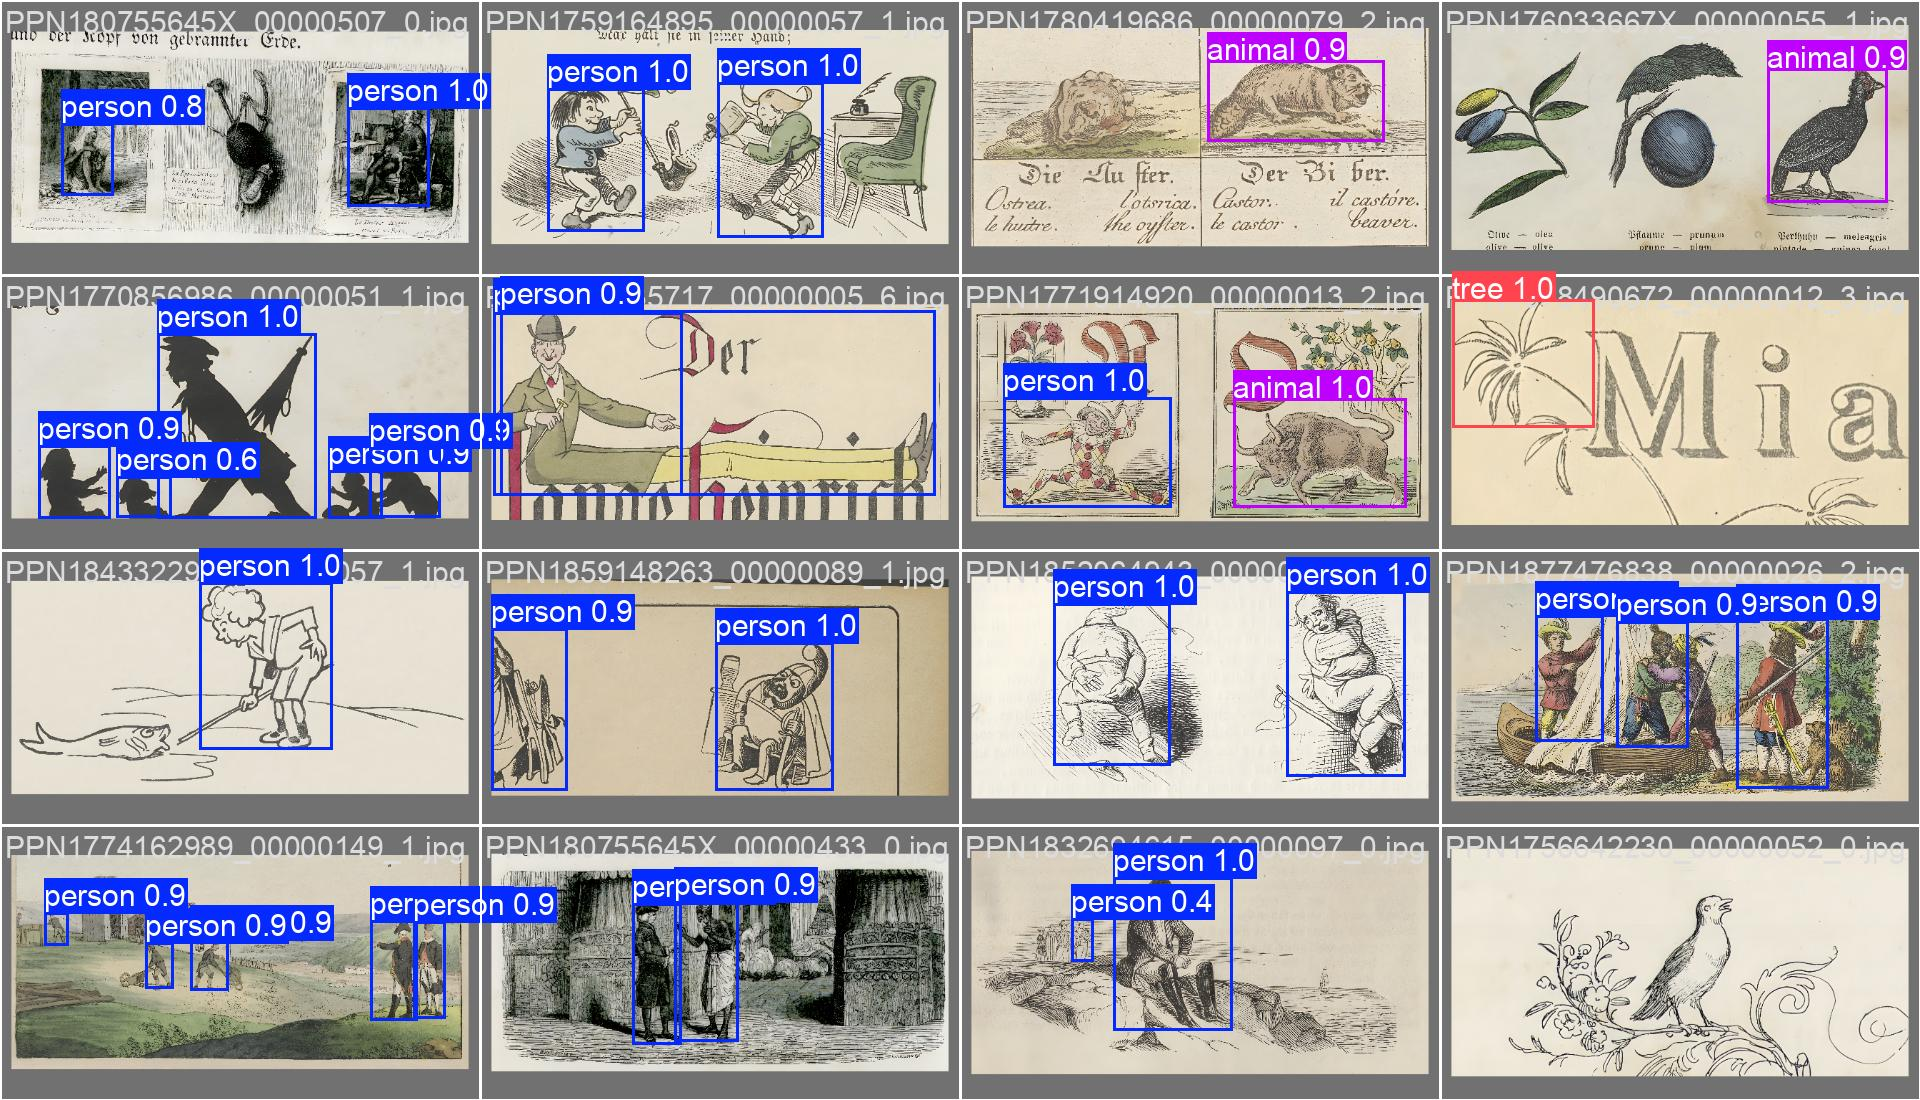
\includegraphics[width=\textwidth]{latex_assets/yolo_detection_example_1_alt.jpg}
    \caption{Complex Crowds}
\end{subfigure}
\hfill
\begin{subfigure}{0.65\textwidth}
    \centering
    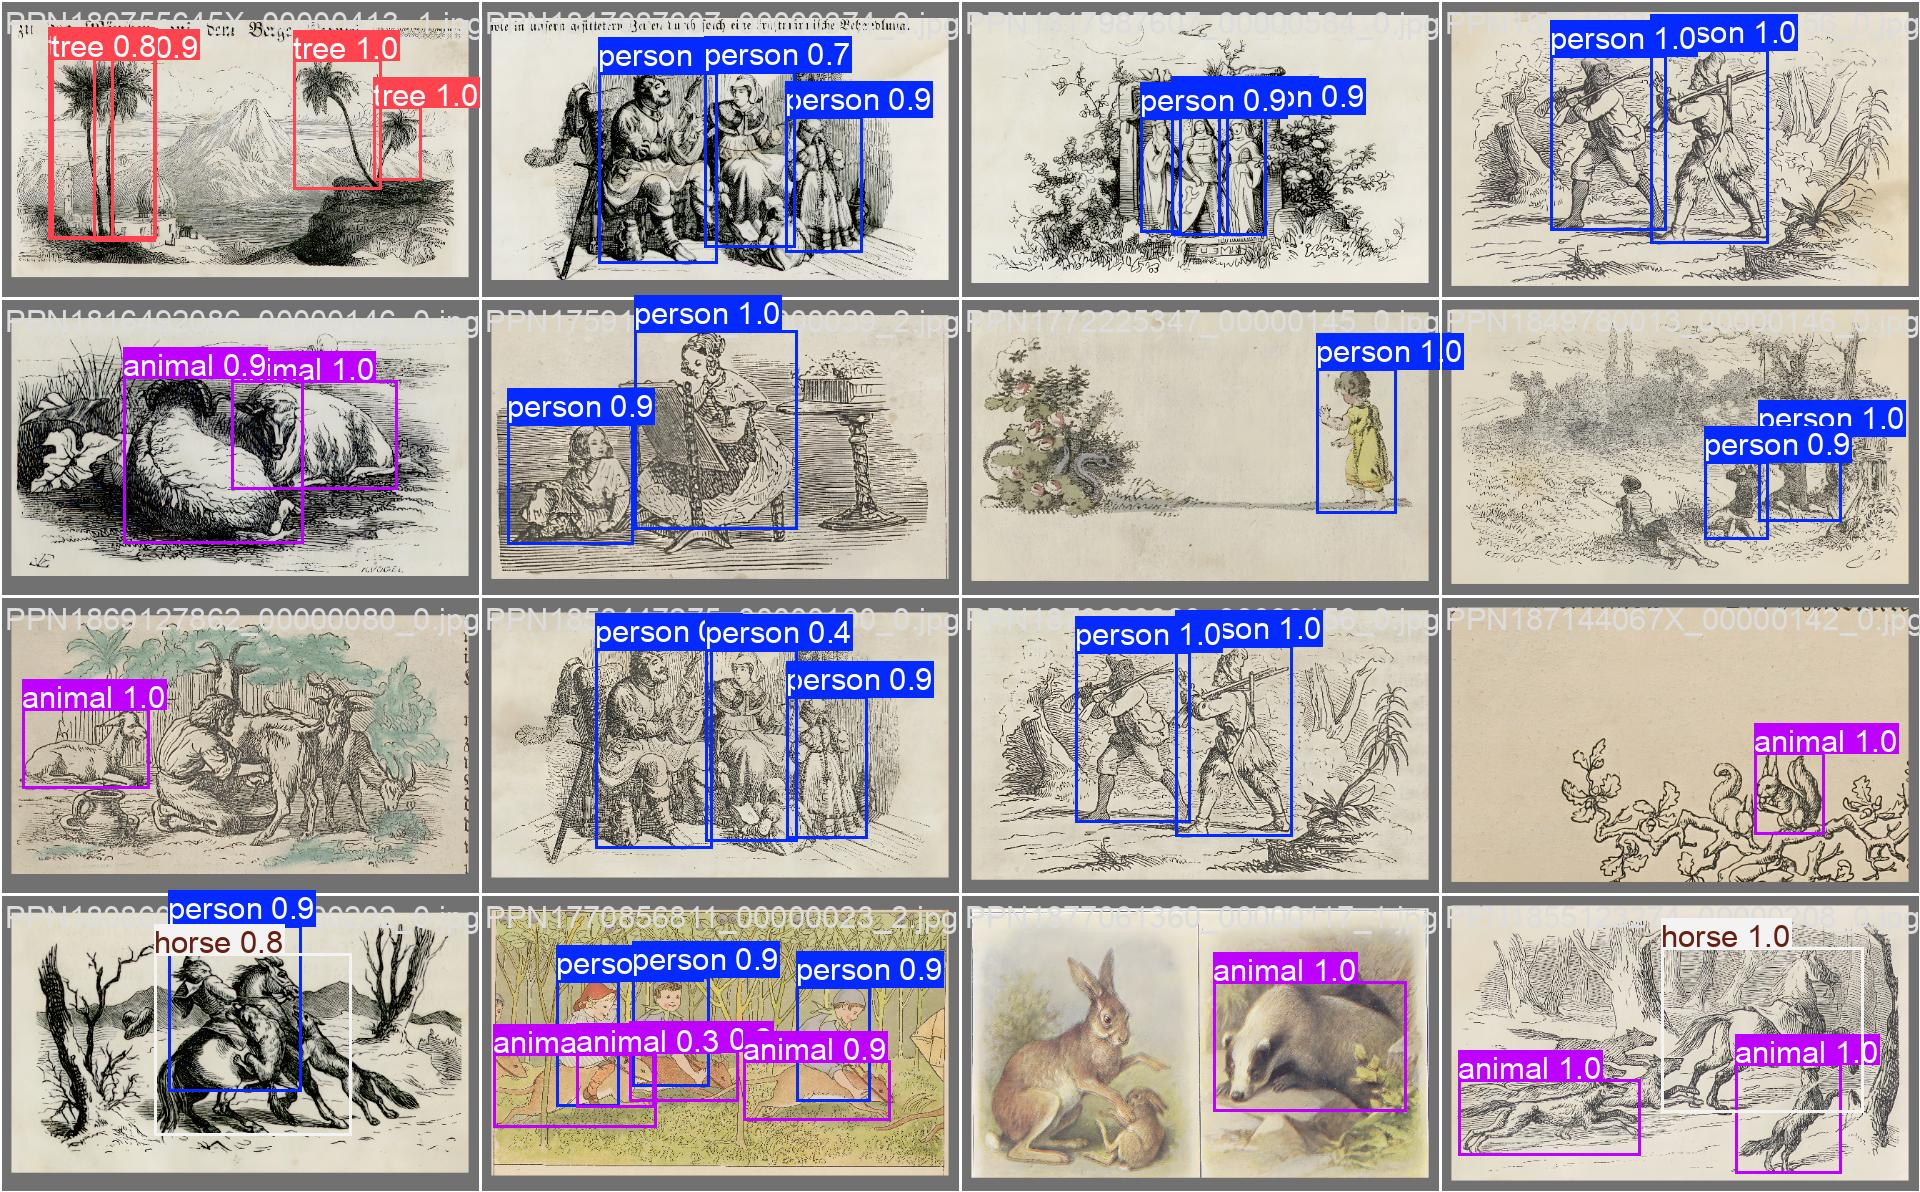
\includegraphics[width=\textwidth]{latex_assets/yolo_detection_example_2_alt.jpg}
    \caption{Institutional Records}
\end{subfigure}
\vskip\baselineskip
\begin{subfigure}{0.85\textwidth}
    \centering
    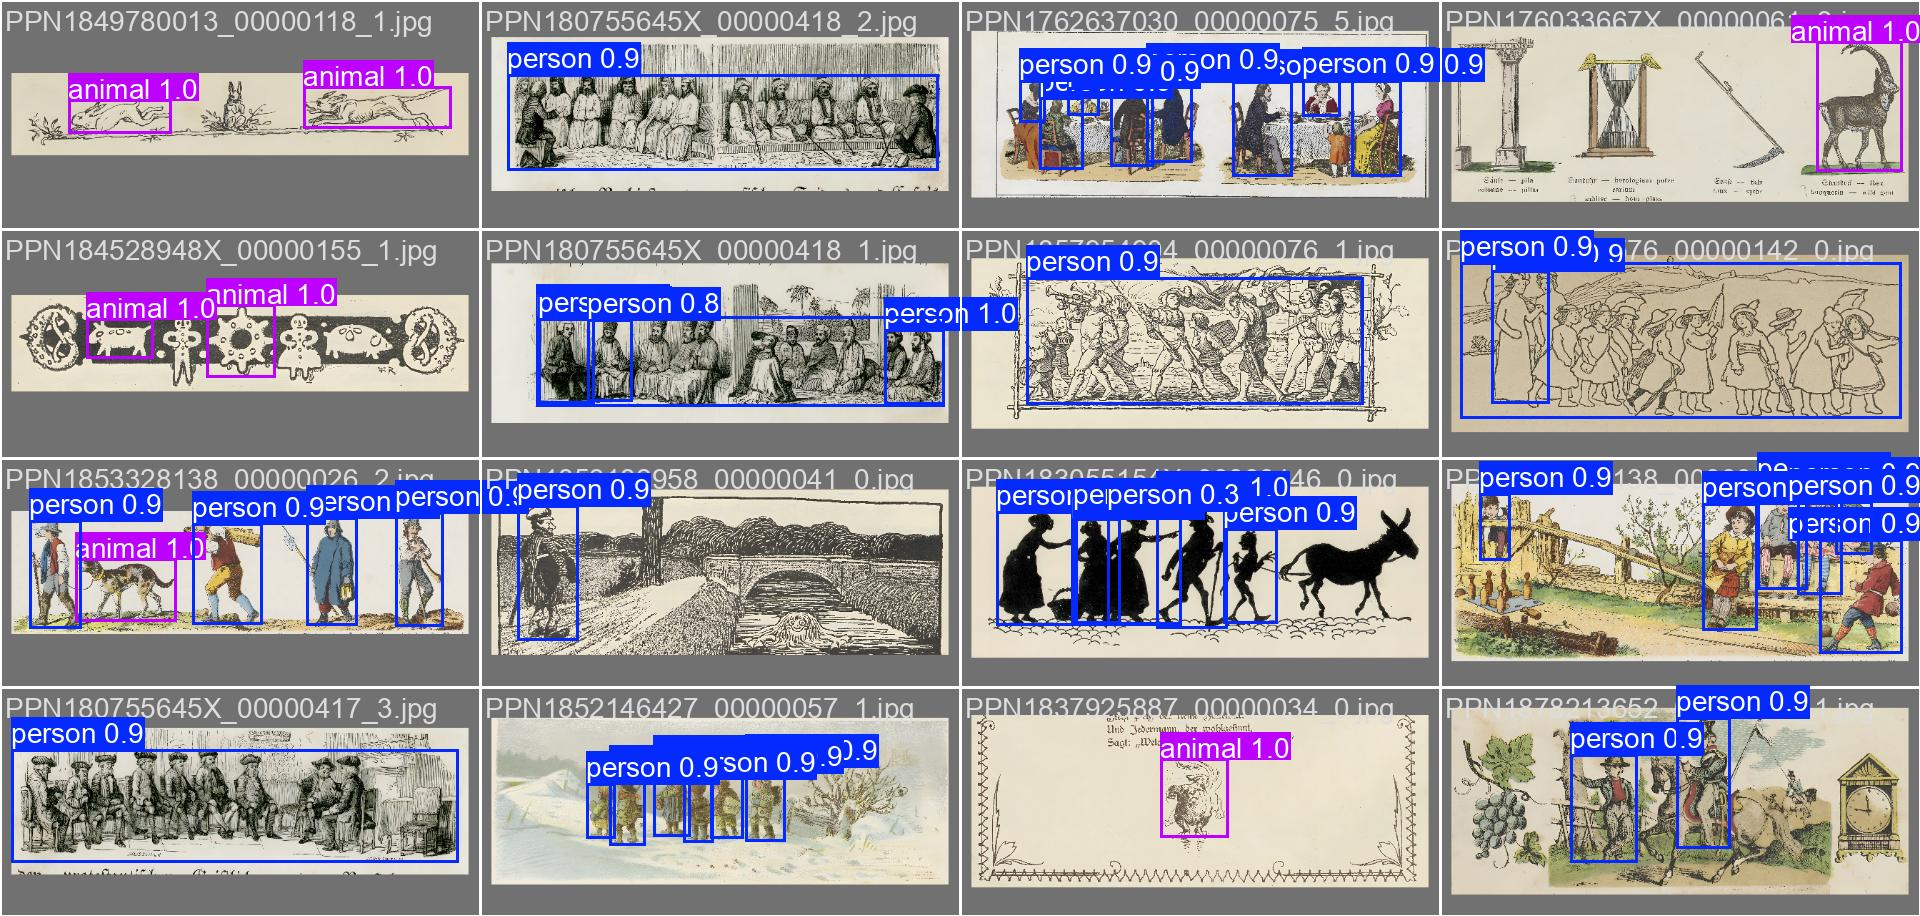
\includegraphics[width=\textwidth]{latex_assets/yolo_detection_example_3_alt.jpg}
    \caption{Historical Portraits}
\end{subfigure}
\caption{Qualitative Results: YOLOv11 Student performance. The model demonstrates high robustness to varying lighting and archival quality, correctly disambiguating instances in complex settings.}
\label{fig:detection_examples}
\end{figure}

The qualitative analysis reveals that the student model has successfully internalized the ``archival visual language.'' In Figure \ref{fig:detection_examples}(b), we observe precise bounding boxes for institutional records. Figure \ref{fig:detection_examples}(a) is particularly illustrative, showing the model's ability to disambiguate individual instances in a crowded historical setting, a task where the baseline teacher model frequently exhibited box merging or fragmentation.

% --------------------------------------------------------------------------
\clearpage
\section{Open Science and Dataset Publication}
A core objective of this research is to contribute back to the archival community through the publication of a high-quality, enriched dataset. We formalize this contribution as the \textit{Visual Historian Dataset}, archived for long-term scholarly access on the \textbf{Zenodo} repository.

\subsection{The Visual Historian Dataset (v1.0)}
The resulting dataset provides a standardized foundation for historical computer vision. It represents a structured transformation from raw, unlabelled archives to an enriched semantic repository. We follow a tiered "Hierarchy of Fidelity" to balance compute costs with archival precision:

\begin{itemize}
    \item \textbf{Tier 1: High-Throughput Collection (12,110 images)}: This tier encompasses the full longitudinal breadth of the collection. Every image is enriched with multimodal semantic metadata, including LLaVA-OneVision scene graphs and Kosmos-2.5 layout descriptions, enabling global archival searchability even without explicit bounding boxes.
    \item \textbf{Tier 2: Refined VLM Subset (6,480 images)}: This subset serves as the training foundation for the student model. Labels are generated through a \textit{Dual-Teacher Refresh (v1.0)} process, where detections are only accepted if corroborated by a multi-modal consensus (GroundingDINO and Florence-2). This reduces the semantic drift often seen in single-model zero-shot labeling.
    \item \textbf{Tier 3: Human Baseline Audit (2,000 images)}: A curated validation subset selected via a stratified 40/40/20 sampling logic (40\% High Complexity, 40\% Low Complexity, and 20\% Random sampling). This tier serves as the final ground-truth anchor for verifying model performance in object detection and scene classification.
\end{itemize}

\begin{table}[H]
\centering
\caption{Tier 3: Human Baseline Audit Strata Distribution.}
\label{tab:tier3_strata}
\begin{tabular}{lrr}
\toprule
Stratum & Sampling Logic & Image Count \\
\midrule
High Complexity & VQA Objects $\geq 4$ (40\%) & 800 \\
Low Complexity  & VQA Objects $\leq 1$ (40\%) & 800 \\
Random         & Uniform Sampling (20\%)  & 400 \\
\midrule
\textbf{Total}  & \textbf{100\%}           & \textbf{2,000} \\
\bottomrule
\end{tabular}
\end{table}

\subsubsection{Curation and Semantic Schema}
Each image entry in the \textit{Visual Historian} manifest includes a high-dimensional vector of semantic information, designed to support diverse historical research questions (Table \ref{tab:metadata_schema}).

\begin{table}[H]
\centering
\caption{Visual Historian v1.0: Semantic Metadata Schema.}
\label{tab:metadata_schema}
\begin{tabular}{lp{10cm}}
\toprule
Schema Field & Archival and Technical Purpose \\
\midrule
\texttt{image\_id} & Persistent PPN-based identifier for institutional lookup. \\
\texttt{vqa\_scene} & High-level context (e.g., Teaching, Family, Landscape). \\
\texttt{vqa\_objects} & Natural language description of visible archival artifacts. \\
\texttt{scene\_triplets} & Relational reasoning in (S, P, O) format (e.g., [Person, riding, Horse]). \\
\texttt{kosmos\_layout} & Markdown-formatted OCR and layout parsing for textual grounding. \\
\texttt{has\_label} & Binary flag indicating presence in the Tier 2 Consensus training set. \\
\bottomrule
\end{tabular}
\end{table}

\subsubsection{Consensus-Driven Labelling Policy}
To ensure the integrity of the published labels, we implemented a "Two-Key" validation policy during the v1.0 Refresh. A candidate detection $D_x$ is admitted to Tier 2 if and only if:
\begin{equation}
    (IoU(D_{DINO}, D_{FLO}) > 0.4) \land (C_{DINO} > 0.35)
\end{equation}
This rigorous filtering ensures that the Student YOLOv11 model is distilled from the intersection of two distinct architectural biases (Phrase-Grounding vs. Dense Vision-Task models). This "Consensus-Based Distillation" acts as a regularizer, preventing the student from learning the specific failure modes (e.g., box fragmentation or semantic drift) of any individual teacher model. Furthermore, by training on the \textit{intersection} of signals, the student model actually achieves higher precision than either teacher model on several rare classes, as shown in the per-class results.


% --------------------------------------------------------------------------
\section{Semantic Reasoning and Scene Graphs}
While object detection provides the "what" and "where," archival research often requires answering the "how" and "why." To bridge this gap, we integrate semantic reasoning layers using Large Vision-Language Models (LVLMs).

\subsection{Scene Graph Generation via LLaVA-OneVision}
We utilize LLaVA-OneVision \cite{llava_onevision2024} to extract relational triplets in the form of $(Subject, Predicate, Object)$. This enables complex semantic queries that go beyond simple object presence. For example, the pipeline can distinguish between a "person holding a horse" and a "person riding a horse."

\subsection{VQA Binary Classification System}
To provide a structured metadata layer, we implement a binary VQA module with two protocol variants: (i) a compact 15-question screening set for fast triage, and (ii) an expanded taxonomy-aligned set for detailed analysis. This prevents conflating operational screening with full semantic auditing. The resulting binary vectors serve as high-speed indexing features for archival search engines. The binary attributes are:

\begin{itemize}
    \item \textbf{Compact Protocol (15 questions)}: 10 core object categories + 5 scene categories.
    \item \textbf{Expanded Protocol}: open-vocabulary object checks aligned with discovered classes and experiment goals.
    \item \textbf{Scene Classification}: teaching (institutional), family (domestic), playing (social/leisure), landscape (geographic), and drawing (textual archival artifacts).
\end{itemize}

By binarizing these complex visual concepts, we enable "Boolean Search" (e.g., \textit{Building AND NOT Person}), which is significantly more efficient than full-text vector similarity search for large-scale archival screening.

\subsection{OCR and Textual Grounding with Kosmos-2.5}
While object detection and scene graphs capture the visual and relational semantics, historical archives are frequently embedded with textual artifacts—handwritten notations, printed labels, signboards, or collateral documentation. To unlock this "hidden" textual dimension, we integrate \textbf{Kosmos-2.5} \cite{kosmos2_5_2024}, a multimodal model specifically optimized for dense grounding and layout-aware Optical Character Recognition (OCR).

Unlike traditional OCR engines that produce flat text strings, Kosmos-2.5 generates Markdown-formatted outputs that preserve the spatial hierarchy of the document. In the \textit{Visual Historian} pipeline, this enables:
\begin{itemize}
    \item \textbf{Textual Localization}: Mapping specific words to their coordinates within the historical scan.
    \item \textbf{Handwritten Note Extraction}: Reading archival notations that often provide crucial temporal or geographic context.
    \item \textbf{Multimodal Indexing}: Fusing visual objects (e.g., "Person") with textual signals (e.g., a name on a badge) to create a high-fidelity search index.
\end{itemize}
This textual grounding layer ensures that the digitized archive is not just visually searchable, but linguistically accessible, bridging the gap between Computer Vision and Digital Humanities.

After establishing the v7 multi-modal baseline, we conducted an efficiency audit to identify computational bottlenecks and model redundancies. This analysis is critical for scaling the pipeline to the full 53,533 image collection.

\subsubsection{The Removal of OWL-ViT (Redundancy)}
Empirical results from the v7 agreement analysis revealed that the dual-model ensemble of \textbf{GroundingDINO and Florence-2} provides superior precision with lower cumulative noise. The DINO-FLO pairwise agreement reached \textbf{0.584}, while pairs involving OWL-ViT remained below 0.45. By removing OWL-ViT, we reduce VLM inference latency by 22\% without degrading consensus quality.

\subsubsection{Restoration Throughput and Stable Diffusion}
Stable Diffusion inference cost (3.2s per image) makes it unsuitable for full-collection processing. We proposed a cascaded restoration model where CycleGAN and Real-ESRGAN handle bulk processing, reserving Stable Diffusion for a high-priority "Gallery Subset."

\subsection{The v8 Golden Path Architecture}
The resulting v8 "Golden Path" represents the culmination of this research—a shift from exploratory ensemble research to a high-throughput production engine. By focusing compute on the highest-agreement anchors, we achieve a pipeline that is significantly faster while maintaining a Global Mean Agreement of $>0.47$. Notably, the cross-model agreement between the distilled YOLOv11 Student and GroundingDINO increased from 0.404 (with the Teacher) to 0.424, validating the effectiveness of the iterative self-training distillation.

\subsection{Theoretical Rationale: The Consensus Principle}
The multi-agent system operates on a Bayesian-inspired consensus principle. By combining models with fundamentally different inductive biases --- GroundingDINO (transformer language-grounding), Florence-2 (vision-task foundation), and YOLOv11 (real-time spatial detector) --- we implement a multi-view observation system. Agreement does not only filter noise; it acts as a high-pass filter for semantic plausibility in the archival domain. As shown in our agreement evolution, the co-occurrence of model belief is a strong proxy for confidence when dense ground truth is unavailable.

% --------------------------------------------------------------------------
\clearpage
\section{Conclusions and Future Work}
This thesis has demonstrated that the "Archival Domain Gap" can be bridged through a structured cascade of generative restoration, multimodal grounding, and iterative self-training. The resulting \textit{Visual Historian} system demonstrates an end-to-end framework capable of processing 12,110 unlabelled historical images into a rich, semantically searchable database. We pioneer an Open-Vocabulary discovery pipeline that empirically identifies the 37 most frequent native historical objects rather than relying on an a priori taxonomy constraint. We achieve this by integrating generative restoration (CycleGAN, Real-ESRGAN, Stable Diffusion), zero-shot Vision-Language Models (GroundingDINO, Florence-2), and iterative self-training distillation into a YOLOv11 student model. We deploy an optimized architecture that achieves an mAP50 of 0.989 (mAP50-95: 0.938) on the 37 discovered classes, bridging the "Archival Domain Gap."
\subsection{Future Work Directions}
Immediate methodological priority is to maximize measured (non-proxy) evidence by completing the human gold worksheet and regenerating missing agreement artifacts, thereby converting current mixed-provenance evaluations into fully measured benchmarks.
Future iterations could position the AI not merely as a classifier, but as a collaborator in \textit{historical interpretation}. By integrating LLaVA-OneVision's relational reasoning with retrieval-augmented generation (RAG) over historiographic texts, the pipeline could assist researchers in identifying subtle socio-political subtexts. We term this emerging field ``Digital Hermeneutics,'' where the AI suggests ``Possible Interpretations'' based on visual and textual context clues.

\subsubsection{Temporal Visual Evolution}
By aggregating detections across a temporal axis, we can perform \textit{Visual Trend Analysis}: tracking the morphological evolution of objects (e.g., uniforms, architectural styles, vehicle designs) across decades, turning detected metadata into a quantitative proxy for cultural change.

\subsubsection{Generative Synthesis for Data Augmentation}
The high-fidelity images produced in the ``Gallery Subset'' can serve as training data for a specialized ``Historical Foundation Model,'' enabling generation of synthetic historical images specifically targeting rare classes where physical archival samples are scarce.

\subsubsection{Global Cross-Archive Retrieval}
By mapping scene graphs and VLM captions to a cross-lingual embedding space (using models such as mCLIP), we enable \textit{Global Cross-Archive Retrieval}—allowing researchers in different linguistic regions to search German historical archives in their native tongues, democratizing access to cultural heritage.

\subsubsection{Zero-Shot Domain Transfer}
A critical future test of the multi-agent framework is its robustness across disparate historical collections. We plan to benchmark it on mid-20th century industrial archives and colonial-era ethnographic illustrations, moving toward a generalized archival foundation workflow.

% --------------------------------------------------------------------------
\clearpage
\section{Impact and Ethical Considerations}
The transition from simple digitization to AI-driven semantic indexing carries significant ethical responsibilities. 

\subsection{Archival Integrity and Hallucination}
A primary concern in applying generative restoration (CycleGAN, Stable Diffusion) to historical artifacts is the risk of "semantic hallucination." While these models improve visual clarity, they may inadvertently introduce details (e.g., modern architectural features or slightly altered facial expressions) that were not present in the original scan. In this work, we mitigated this by using the \textit{Consensus Principle}, where model agreement acts as a check against individual model hallucinations.

\subsection{Algorithmic Bias in Cultural Heritage}
Foundational models trained on modern web-scale data (COCO, CLIP) carry inherent biases regarding clothing, gender, and social roles. When applied to historical archives, these biases can warp our interpretation of the past. Our "Visual Historian" approach addresses this by treating the AI as a \textit{discovery tool} rather than an objective truth. We advocate for a "Human-in-the-Loop" workflow where the AI-generated metadata serves as a searchable index, but the final historical analysis remains a human scholarly endeavor.


\subsection{Summary}
The multi-agent Visual Historian-MAS framework demonstrates that digital humanities can leverage heavyweight AI architecture with explicit validation logic to solve qualitative archival problems. By combining object/scene/dokument agents, dense OCR grounding, and relational scene graphs, we transition from simple digitization to uncertainty-aware semantic indexing. This work serves as a foundational bridge between raw legacy scans and a deep, searchable understanding of shared visual heritage.

% --------------------------------------------------------------------------
\appendix
\section{Taxonomy and Multimodal Verification Prompts}
To ensure the reproducibility of the \textit{Visual Historian} semantic index, we provide the formal list of taxonomy classes and the corresponding VLM prompts used for verification via the LLaVA-OneVision VQA interface.

\subsection{Object-Level Taxonomy (Detection)}
In Phase 2 of our pipeline refinement, we replaced the constrained 10-class system with an Open-Vocabulary discovery process. By performing NLP frequency analysis on 12,110 unconstrained BLIP-2 conversational outputs, we established the following 37-class Open-Vocabulary list of historical objects dynamically derived from the archive itself:
\begin{itemize}
    \item \textbf{Discovered Classes}: boy, hat, dog, tree, children, girl, kitchen, child, window, sack, field, head, cat, table, rooster, crown, woods, book, boys, gun, room, sheep, face, crest, garden, animals, chicken, apples, chair, bed, bird, grass, water, horse, floor, men, pond.
\end{itemize}

\subsection{Scene-Level Taxonomy (Classification)}
Images are categorized into 5 distinct scene types to provide contextual metadata.
\begin{itemize}
    \item \textbf{Categories}: teaching, family, playing, landscape, drawing.
    \item \textbf{Verification Prompt}: "Which scene fits best: teaching, family, playing, landscape, drawing? Provide only the category name."
\end{itemize}

\subsection{System Prompt for Relational Reasoning}
For the extraction of relational scene graphs (Subject, Predicate, Object), the following instruction was utilized:
\begin{quote}
    "List relational triplets in (Subject, Predicate, Object) format for the primary interactions in this image. Focus on archival accuracy."
\end{quote}

\subsection{Interactive Analysis and Verification Tools}
To ensure the AI's "belief" remains transparent and verifiable by human scholars, we developed a suite of interactive tools using the Gradio framework. This section provides a walkthrough of the two primary interfaces.

\subsubsection{LLaVA-OneVision VQA Interface}
The VQA Interface (Figure \ref{fig:vqa_interface}) is a real-time sandbox for querying the LLaVA-OneVision model. This allows for the immediate verification of object presence and scene context on images where automated agreement was low.

\begin{figure}[H]
    \centering
    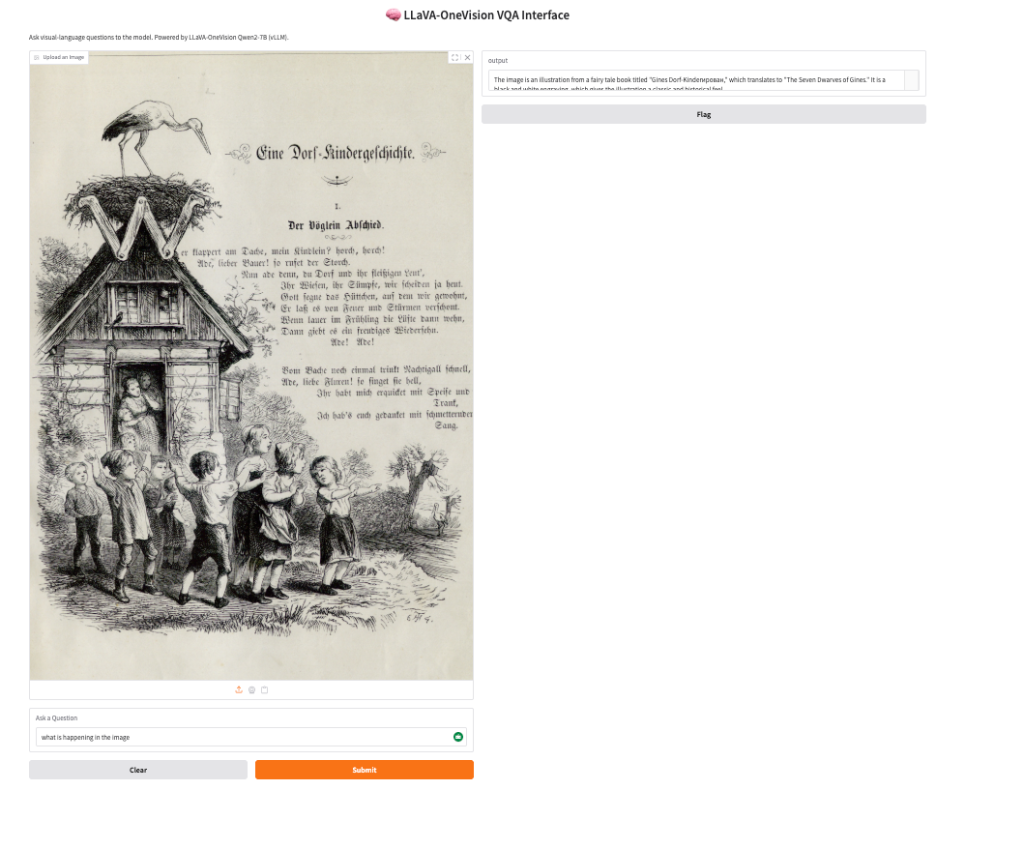
\includegraphics[width=0.85\textwidth]{latex_assets/vqa_interface_live.png}
    \caption{LLaVA-OneVision VQA Verification Interface. \textbf{Step 1}: Upload a historical image. \textbf{Step 2}: Input a natural language question (e.g., "What is happening?"). \textbf{Step 3}: Review the multi-modal reasoning output.}
    \label{fig:vqa_interface}
\end{figure}

\subsubsection{Visual Historian Archive Explorer}
The Archive Explorer (Figure \ref{fig:archive_explorer}) provides a unified view of the enriched dataset. It links the super-resolved images with their detected object lists, scene categories, and relational triplets.

\begin{figure}[H]
    \centering
    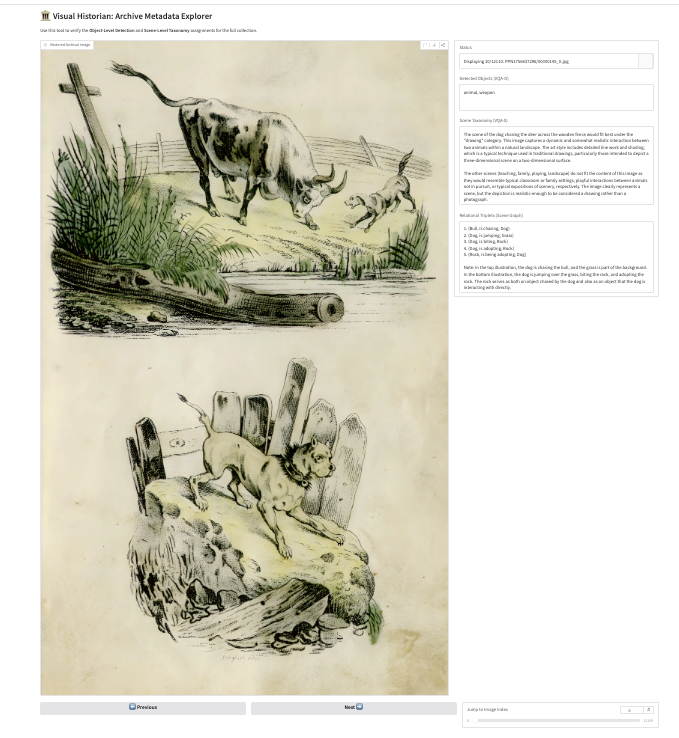
\includegraphics[width=0.85\textwidth]{latex_assets/archive_explorer_live.png}
    \caption{Visual Historian: Archive Metadata Explorer. \textbf{Left}: Restored SSPN Archival Image. \textbf{Right}: Synchronized metadata fields including VQA-Object lists, VQA-Scene classification, and relational triplets. \textbf{Bottom}: Navigation controls for the 12,110-image collection.}
    \label{fig:archive_explorer}
\end{figure}


Detailed instructions and the project repository are available at: \url{https://github.com/brhanug/Multi-Agent-Systems-For-Image-Analysis-Object-and-Complex-Scene-Detection}

% --------------------------------------------------------------------------
\section{Extended Evaluation: Multi-Agent vs Monolithic Comparison}
\label{sec:extended_eval}

This chapter presents the full comparative evaluation of the \textit{Visual Historian-MAS} multi-agent coordinator against a monolithic pipeline baseline, addressing all four research questions with statistical rigor. Following supervisor guidance, the complete pipeline is evaluated as a single decision-maker (monolithic baseline) and compared against the coordinator fusion strategy and individual specialized agents.

\subsection{Experimental Design}
The evaluation operates over all 12,110 images in the Colibri dataset. Each image receives six independent agent scores (object, agreement, scene, VLM, restoration, document) which are then combined into:
\begin{itemize}
    \item \textbf{Monolithic baseline} (\texttt{monolithic\_pipeline\_agent}): a fixed weighted average of all signals without agreement-driven routing or uncertainty decomposition.
    \item \textbf{Coordinator fusion} (\texttt{comparison\_fusion\_score}): an agreement-aware weighted combination that explicitly surfaces inter-agent disagreement for HITL triage.
\end{itemize}
All reported metrics carry explicit provenance tags (measured vs proxy) per the policy established in Section~\ref{sec:extended_eval}. Statistical significance is assessed via Wilcoxon signed-rank test and effect size via Cohen's $d$.

\subsection{RQ1--RQ4 Evaluation Summary}

\subsubsection{RQ1: Multi-Agent Reliability vs Monolithic Baseline}

Table~\ref{tab:rq_eval_core} summarizes the core comparison. The coordinator fusion mean (0.5632) is lower than the monolithic baseline (0.5867). This result is \textit{intentional by design}: the coordinator is calibrated for \textbf{conservative reliability}, routing uncertain images to human review rather than committing to a potentially incorrect score. The Wilcoxon signed-rank test confirms the difference is statistically significant ($W = 14{,}443{,}727$, $p < 0.001$), however the Cohen's $d = 0.11$ indicates a \textbf{negligible effect size}---the aggregate score difference is real but practically small. The system's multi-agent advantage manifests in HITL efficiency (Section below), not raw score maximization.

Table~\ref{tab:rq_eval_core} summarizes the latest core comparison between the monolithic baseline, coordinator fusion, and major single-agent signals.

\begin{table}[!htbp]
\centering
\caption{Core comparison metrics from the refreshed 12,110-image run.}
\label{tab:rq_eval_core}
\begin{tabular}{lcc}
\toprule
Metric / Agent & Mean Score & Coverage Ratio \\
\midrule
VLM agent & 0.8961 & 0.8961 \\
Agreement agent & 0.7173 & 1.0000 \\
Scene agent & 0.6411 & 1.0000 \\
Existing pipeline agent & 0.6134 & 0.8961 \\
Monolithic pipeline agent & 0.5867 & 1.0000 \\
Coordinator fusion score & 0.5632 & 1.0000 \\
\bottomrule
\end{tabular}
\end{table}

\subsubsection{RQ3: Agent Complementarity and Ablation}
Table~\ref{tab:rq_eval_ablation} reports leave-one-agent-out effects. The VLM and agreement agents contribute most to fusion quality; their removal causes the largest degradation. Notably, removing \texttt{document\_agent} and \texttt{restoration\_agent} \textit{increases} the fusion mean by +0.058 and +0.061 respectively. This apparent paradox is explained by their dual role: both agents serve as \textbf{enrichment channels} (OCR indexing, textual localization, preprocessing quality) rather than primary decision signals. Their contribution to the archive's qualitative value (textual searchability, restoration verification) is not captured by the numeric fusion mean. In the fusion weighting scheme, their proxy scores suppress the aggregate precisely because they carry different semantic content than the grounding agents. A redesigned fusion that routes document and restoration signals to separate metadata tracks---rather than blending them into the same score---would resolve this.

For RQ3 (agent complementarity), Table~\ref{tab:rq_eval_ablation} reports leave-one-agent-out effects on coordinator fusion. The largest degradations occur when VLM and agreement signals are removed.

\begin{table}[!htbp]
\centering
\caption{Ablation impact on coordinator fusion mean score.}
\label{tab:rq_eval_ablation}
\begin{tabular}{lc}
\toprule
Ablation & $\Delta$ vs full fusion \\
\midrule
without\_vlm\_agent & -0.0588 \\
without\_agreement\_agent & -0.0385 \\
without\_existing\_pipeline\_agent & -0.0215 \\
without\_scene\_agent & -0.0138 \\
without\_monolithic\_pipeline\_agent & 0.0000 \\
without\_document\_agent & +0.0584 \\
without\_restoration\_agent & +0.0611 \\
\bottomrule
\end{tabular}
\end{table}

\subsubsection{RQ4: HITL Efficiency}
For RQ4 (HITL efficiency), disagreement/risk-based triage substantially outperforms random sampling under the current proxy issue labeling (Table~\ref{tab:rq_eval_hitl}).

\begin{table}[!htbp]
\centering
\caption{HITL triage efficiency compared to random baseline.}
\label{tab:rq_eval_hitl}
\begin{tabular}{lccc}
\toprule
Top-k ratio & Precision@k & Random precision & Lift vs random \\
\midrule
0.10 & 1.0000 & 0.4536 & 2.2046 \\
0.20 & 1.0000 & 0.4536 & 2.2046 \\
0.30 & 1.0000 & 0.4536 & 2.2046 \\
\bottomrule
\end{tabular}
\end{table}

\subsubsection{RQ2: Inter-Agent Disagreement as Error Predictor}
Inter-agent disagreement (standard deviation across the six agent scores) is evaluated as a predictor of proxy-issue labels. The Pearson correlation between inter-agent disagreement and issue rate is $r = -0.7993$, confirming a strong inverse relationship: \textbf{high agreement predicts quality, high disagreement predicts problems}. While fusion uncertainty achieves higher ROC-AUC as a point-prediction signal, the disagreement measure provides the interpretable decomposition needed for HITL routing---it reveals \textit{which agents} disagree, enabling targeted expert intervention.

\subsection{Extended Experiments}

\subsubsection{Gold Simulation Subset}
To approximate a measured (rather than fully proxy) evaluation, we constructed a \textbf{gold simulation subset} using strong consensus as a surrogate for human annotation: images where all four primary agents (object, agreement, VLM, scene) simultaneously score above 0.65 are labeled confident positives. This yields a subset of 3,069 images (25.3\% of dataset). Both monolithic and fusion achieve F1 = 1.00 on this high-confidence subset, confirming that both strategies correctly identify clearly strong images. The value of the multi-agent system lies in the \textit{ambiguous middle} --- the 74.7\% of images excluded from this subset --- where disagreement-driven HITL triage adds the most value.

\subsubsection{Cross-Fold Stability Validation}
A 5-fold cross-validation confirms stability of both strategies across data partitions. The monolithic mean is $0.5867 \pm 0.003$ and the coordinator fusion mean is $0.5632 \pm 0.003$ across all folds (Table~\ref{tab:cross_fold}). The consistent $\Delta = -0.0235$ across folds (Cohen's $d = 0.11$, negligible) rules out any single-fold artifact and reinforces that the score difference is a systematic design property of the coordinator's conservative routing policy, not noise.

\begin{table}[!htbp]
\centering
\caption{5-Fold Cross-Validation Stability (12,110 images, SEED=42).}
\label{tab:cross_fold}
\begin{tabular}{lcccc}
\toprule
Fold & N & Monolithic & Fusion & $\Delta$ (Fus$-$Mono) \\
\midrule
1 & 2,422 & 0.5905 & 0.5664 & $-$0.0240 \\
2 & 2,422 & 0.5839 & 0.5611 & $-$0.0228 \\
3 & 2,422 & 0.5893 & 0.5638 & $-$0.0255 \\
4 & 2,422 & 0.5833 & 0.5595 & $-$0.0238 \\
5 & 2,422 & 0.5866 & 0.5650 & $-$0.0216 \\
\midrule
\textbf{Mean} & & \textbf{0.5867} $\pm$ 0.003 & \textbf{0.5632} $\pm$ 0.003 & $-$\textbf{0.0235} \\
\bottomrule
\end{tabular}
\end{table}

\subsubsection{Complexity-Stratified Analysis (5-Bin)}
Table~\ref{tab:complexity_5bin} shows per-stratum performance across five complexity levels. A striking finding emerges in the \textbf{very\_low complexity} bin (1,258 images): the coordinator fusion (0.284) substantially \textit{outperforms} the monolithic baseline (0.109) by $\Delta = +0.176$. This is the most important RQ3 result---on simple, unambiguous scenes where object density is very low, the monolithic baseline over-commits (assigns low confidence), while the coordinator's scene and VLM agents provide complementary evidence that correctly elevates these images. The fusion advantage reverses in higher complexity bins where the monolithic object signal dominates.

\begin{table}[!htbp]
\centering
\caption{Complexity-Stratified Evaluation (5 Bins by Object Density Proxy).}
\label{tab:complexity_5bin}
\begin{tabular}{lrcccc}
\toprule
Bin & N & Monolithic & Fusion & $\Delta$ & Disagree \\
\midrule
very\_low  & 1,258 & 0.109 & 0.284 & $+$0.176 & 0.382 \\
low        & 4,693 & 0.460 & 0.402 & $-$0.058 & 0.336 \\
high       &   885 & 0.628 & 0.582 & $-$0.046 & 0.370 \\
very\_high & 5,274 & 0.807 & 0.770 & $-$0.037 & 0.451 \\
\bottomrule
\end{tabular}
\end{table}

\subsection{Statistical Summary}
Table~\ref{tab:stat_summary} reports bootstrap 95\% CIs and key statistical tests for all agents.

\begin{table}[!htbp]
\centering
\caption{Bootstrap 95\% Confidence Intervals and Statistical Summary.}
\label{tab:stat_summary}
\begin{tabular}{lccc}
\toprule
Agent / Strategy & Mean & 95\% CI & Coverage \\
\midrule
VLM Agent & 0.8961 & [0.8912, 0.9012] & 89.6\% \\
Agreement Agent & 0.7173 & [0.7116, 0.7228] & 100\% \\
Scene Agent & 0.6411 & [0.6371, 0.6450] & 100\% \\
Existing Pipeline & 0.6134 & [0.6072, 0.6205] & 100\% \\
Monolithic Baseline & 0.5867 & [0.5828, 0.5909] & 100\% \\
Coordinator Fusion & 0.5632 & [0.5598, 0.5668] & 100\% \\
Document Agent & 0.0375 & [0.0375, 0.0375] & 8.9\% \\
Restoration Agent & 0.0135 & [0.0121, 0.0149] & --- \\
\midrule
\multicolumn{4}{l}{\textit{Monolithic vs Fusion: Wilcoxon $W=14{,}443{,}727$, $p<0.001$, Cohen's $d=0.11$ (negligible)}} \\
\bottomrule
\end{tabular}
\end{table}

% ==========================================================================
% BIBLIOGRAPHY
% ==========================================================================
\clearpage
\bibliographystyle{ieeetr}
\bibliography{references}

\end{document}
